\chapter{Results}
\label{ch:results}

This chapter presents the results of the project to address our research question:
\begin{mainbox}{} 
      \textit{How can design theories and principles of information visualization, combined with an iterative development process, be applied to improve the usability and functionality of a website monitoring dashboard? }
\end{mainbox}
The results comprise of qualitative and quantitative results from user testing, as well as all requirements that were elicited and implemented in accordance with the process outlined in \autoref{sec:req_gathering}. The chapter aims to show the how the monitoring dashboard evolved throughout the iterative development process.

\section{Requirements Prior to User Testing}
Requirement gathering occurred in three stages as described in \autoref{sec:req_gathering}. The first stage involved analysing the assignment brief provided by Headspin, and a subsequent clarification meeting where the brief was further discussed. \autoref{tab:stakeholder_functional_res} and \autoref{tab:stakeholder_nonfunc_res} show the requirements gathered from this first stage. The prototype used in user test 1 was created based on these requirements.

\begin{table}[H]
\centering
\begin{tabular}{| l  |p{0.6\textwidth}  |l |} 
\hline
\textbf{ID} & \textbf{Requirement Description}& \textbf{Priority} \\ \hline
F.1 & User can add, edit and delete monitored websites via the user interface.& High \\ \hline
F.2 & User can set custom check interval per site.& High \\ \hline
F.3 & Display HTTP status, response time, and uptime history for each website.& High \\ \hline
F.4 & Verify that a site is actually up (beyond HTTP 200). & High \\ \hline 
F.5 & Trigger alerts and notifications via e-mail or sms.&Medium \\ \hline
F.6 & Implement user authentication with personalized dashboards.& Medium\\ \hline
F.7 & Add functionality for filtering and sorting of websites.& Medium \\ \hline
\end{tabular}
\caption{Functional requirements (after stakeholder meeting)}
\label{tab:stakeholder_functional_res}
\end{table}

\begin{table}[H]
\centering
\begin{tabular}{| l  |p{0.6\textwidth}  |l |} 
\hline
\textbf{ID} & \textbf{Requirement Description} & \textbf{Priority} \\ \hline
NF.1 & Support monitoring of 50+ sites without noticeable delay.& High \\ \hline
NF.2 & Website status changes must be easy to interpret at a glance. & High \\ \hline
NF.3 & Interface must be user‑friendly and intuitive. & High \\ \hline
NF.4 & Code base should be maintainable and documented. & Medium \\ \hline
NF.5 & Application must adhere to universal design principles & Low \\\hline
\end{tabular}
\caption{Non‑functional requirements after stakeholder meeting}
\label{tab:stakeholder_nonfunc_res}
\end{table}

These requirements were further refined, expanded on, and implemented as described in \autoref{sec:user_test_results}.



\section{User Interfaces Evaluated in User Testing}
\label{sec:artefact_snapshot}

This section details the two versions of the monitoring dashboard that were used to gather feedback in user test 1 and 2. \autoref{fig:dashboards_comparison} shows an overview of the dashboard page from the prototype compared to the \achshort{mvp}.


\begin{figure}[H]
    \centering
    \makebox[\textwidth][c]{%
        \begin{minipage}{1.2\textwidth}
            \centering
            \begin{subfigure}{0.49\textwidth}
                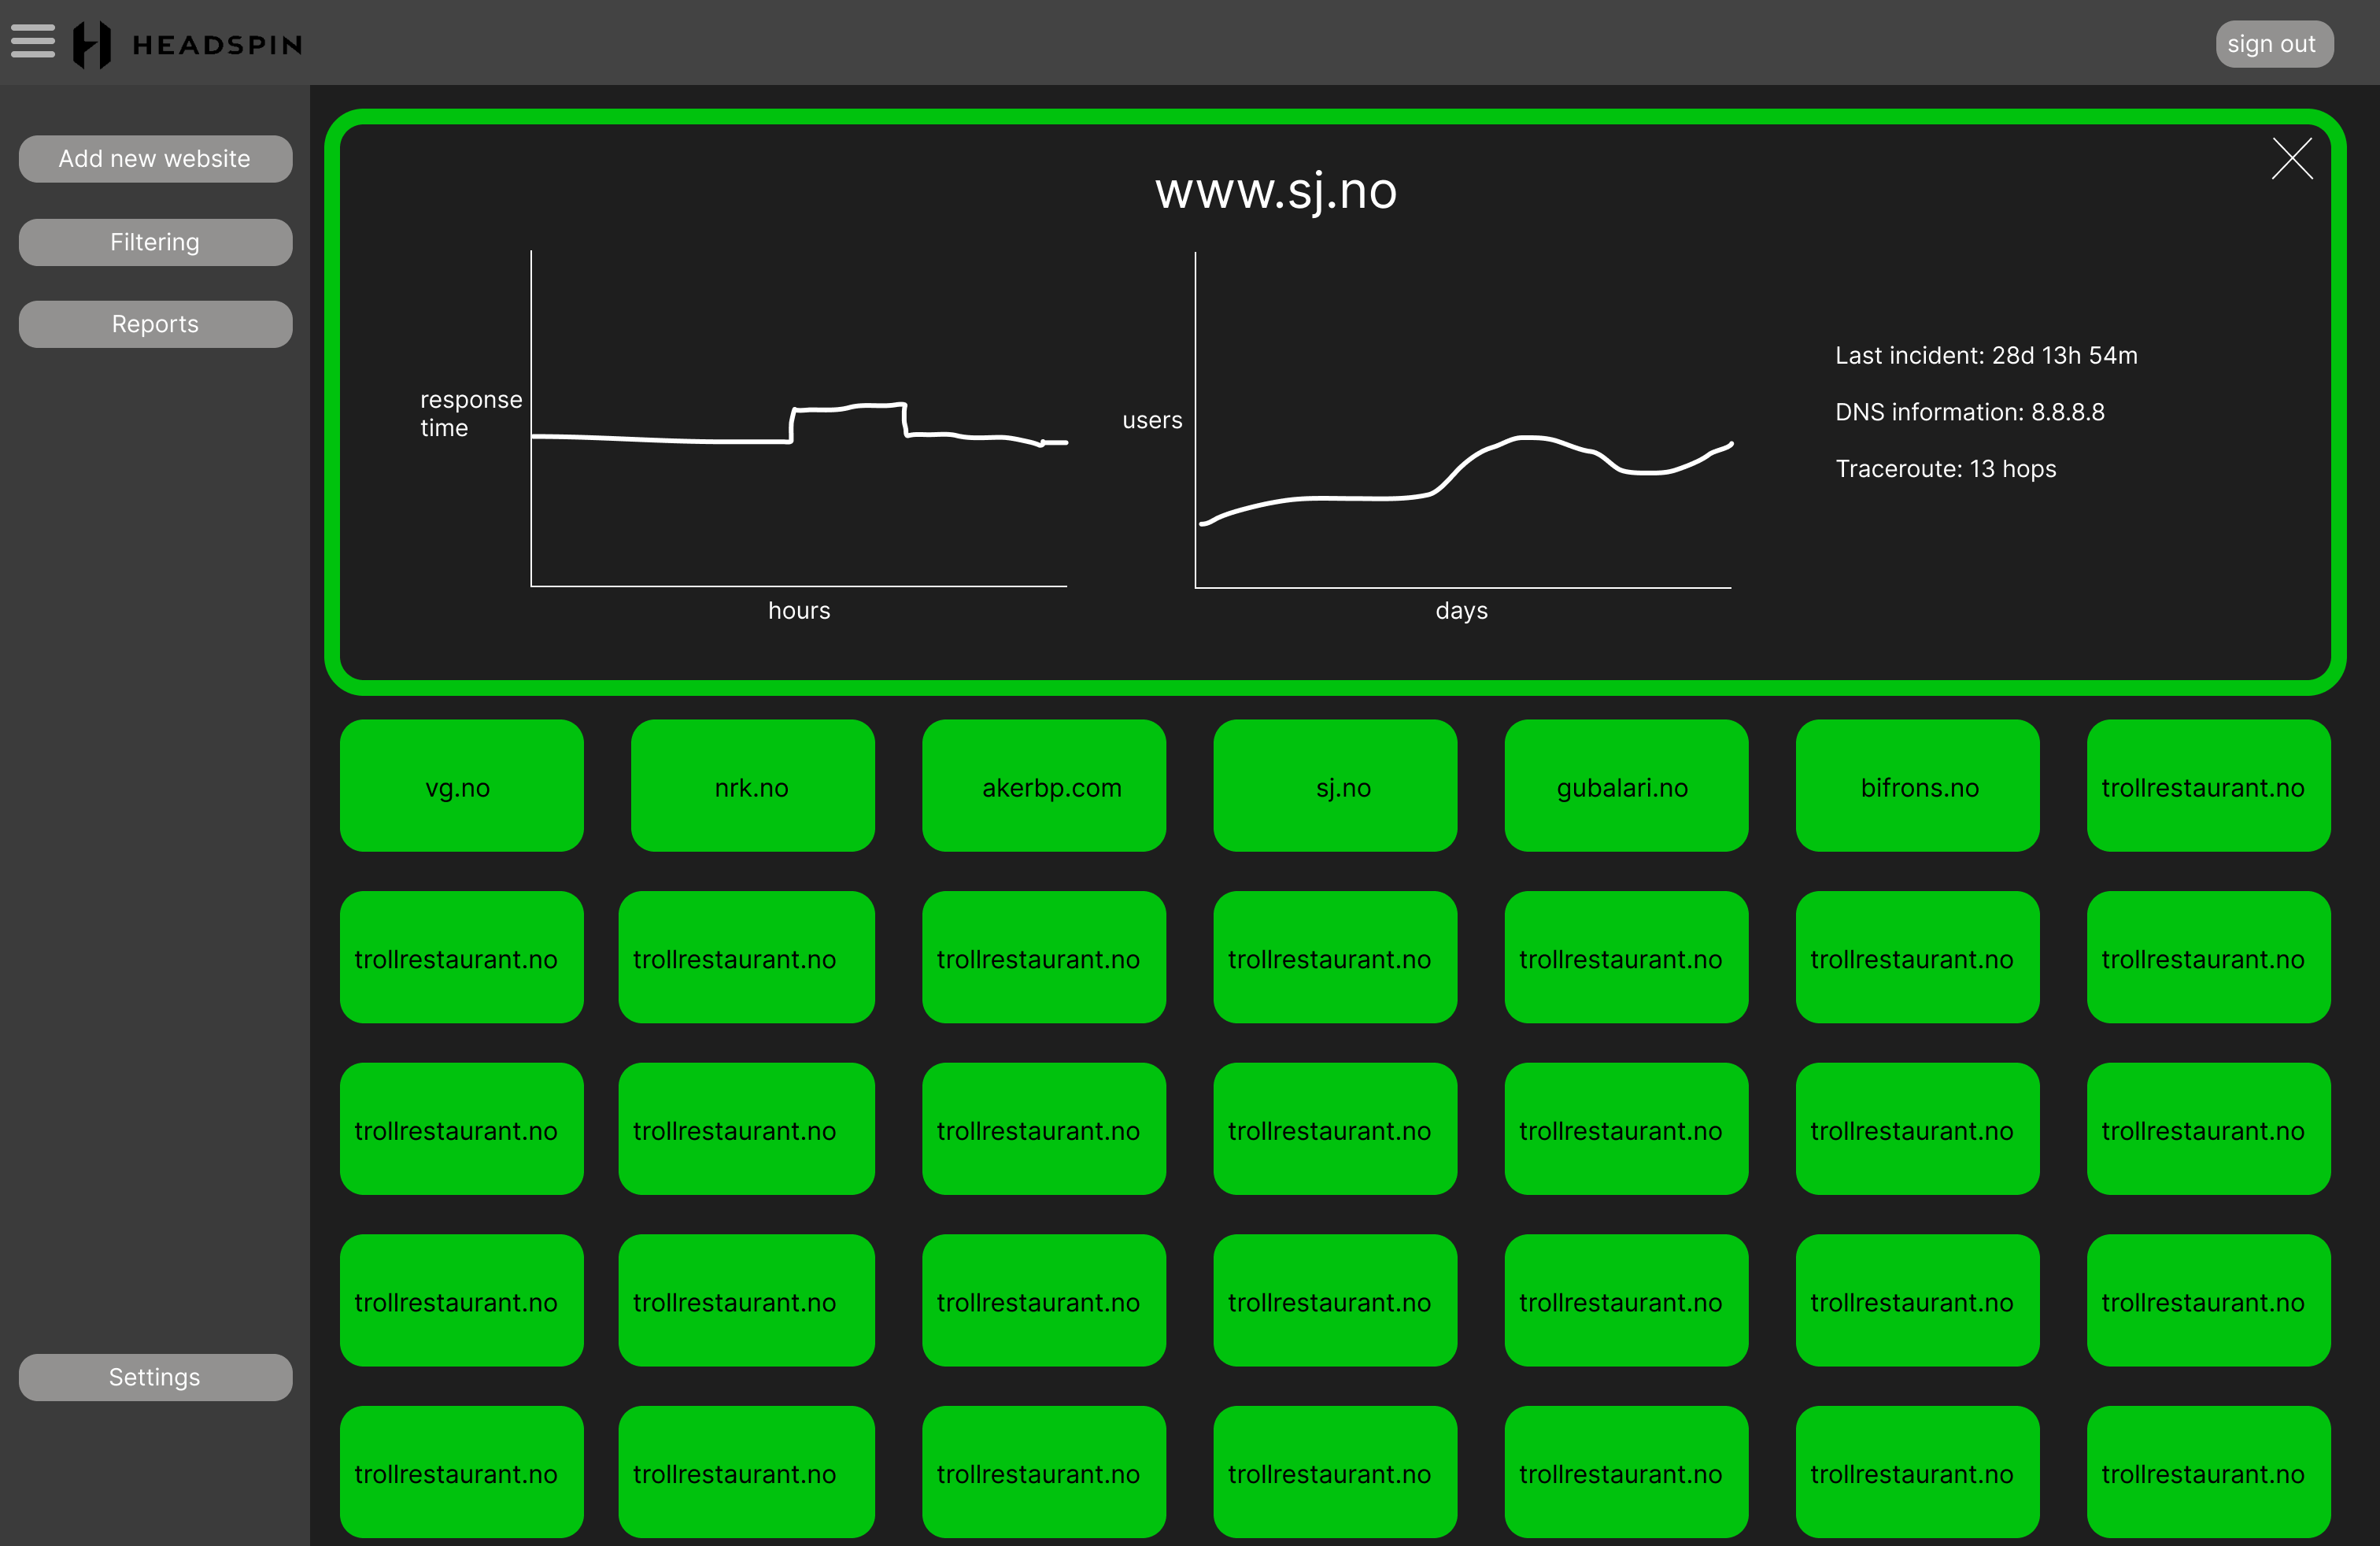
\includegraphics[width=\linewidth]{figures/prototype/prototype_dashboard.png}
                \caption{Prototype dashboard (User Test 1)}
                \label{fig:prototype_dashboard}
            \end{subfigure}
            \hfill
            \begin{subfigure}{0.49\textwidth}
                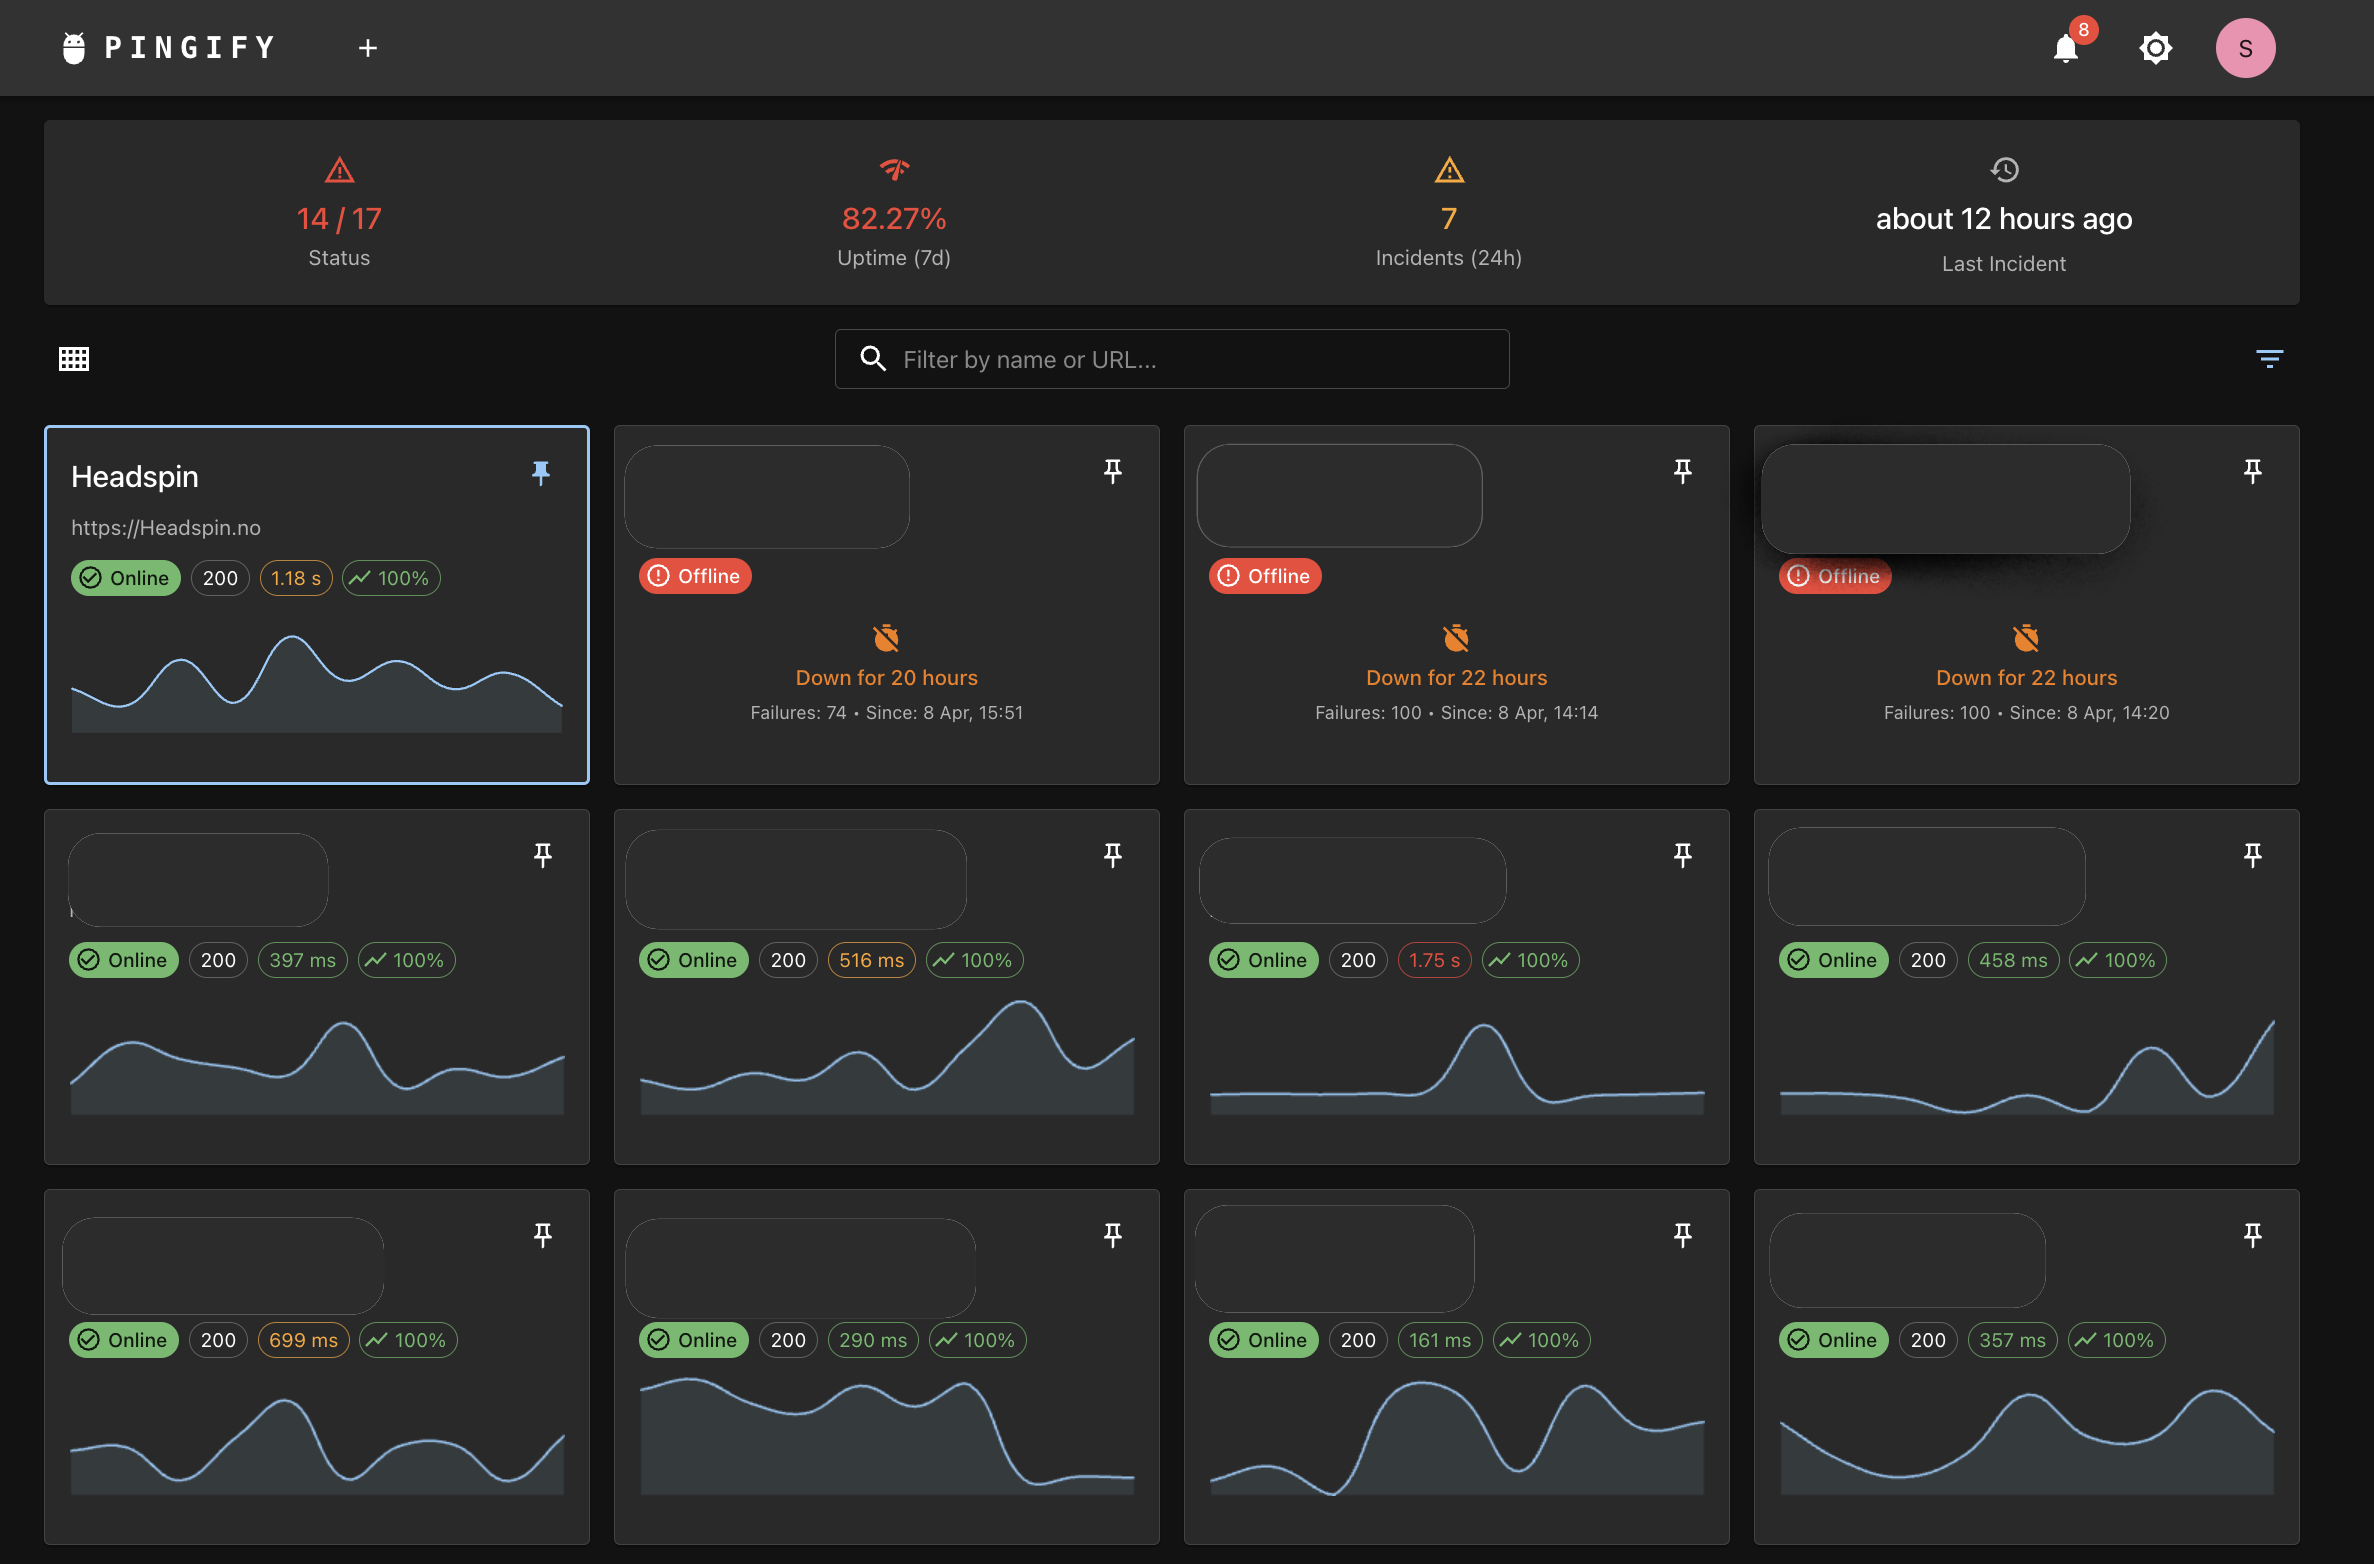
\includegraphics[width=\linewidth]{figures/MVP-dashboard/MVP-dash.png}
                \caption{MVP dashboard (User Test 2)}
                \label{fig:mvp_dashboard}
            \end{subfigure}
        \end{minipage}
    }
    \caption{Comparison of prototype and MVP dashboard pages}
    \label{fig:dashboards_comparison}
\end{figure}

\paragraph{Prototype}
The prototype was designed to comply with functional requirements from the stakeholder clarification meeting. (see \autoref{tab:stakeholder_functional_res}). The prototype consists of a grid of cards to display the status of monitored websites by changing the colour of each card based on if the website is up or down. This addresses F.3. When a card is clicked, the card expands into a detailed view showing graphs and data for that specific website also answers requirement F.3. It also included a collapsible sidebar with different buttons, such as "Add website", "Filtering", "Settings" and "Profile", which addresses requirement F.1, F.2 and F.7. The navigation bar consisted of a logo and a "Sign out"-button, the button navigated the user to a simple login page, showing functionality for requirement F.6. 

The functionality in the prototype was only conceptual and was implemented by navigating between different pages of the prototype with small changes on each page to show how it was intended to function. For a full overview of the prototype, see \autoref{app:prototype_figures}.


\section{Results From User Testing}
\label{sec:user_test_results}
This section addresses findings related to our research question by presenting both qualitative and quantitative results from user test 1 and 2. We describe how user feedback directly influenced the design of the dashboard throughout the iterative development process, that was explained in \autoref{ch:methodology}.

\subsection{Qualitative results}
The qualitative results are based on structured observations and written notes from user tests 1 and 2, in which three employees from Headspin participated. Each participant completed both test rounds, interacting first with the prototype and later with the MVP, followed by semi-structured interviews aimed at uncovering usability issues and improvement opportunities. The findings are presented chronologically, starting with feedback from user test 1, followed by the design changes implemented prior to user test 2. Next, we present the feedback from user test 2 and how this was used in further refinements. Throughout this process, we highlight specific requirements that were added or revised based on user feedback during both testing phases.


\subsubsection{Feedback from Prototype (User Test 1)}  
All participants found the website cards too sparse in information. Participant 1 (P1) requested additional data, such as response time in milliseconds and uptime percentages over different time spans (day, month, year), to be shown directly on the cards (Requirement F.8 \autoref{tab:f_req_usertest_1}). Participant 3 (P3) found the interface clear at first glance, but also reflected that the cards showed too little information. 

P1 also wanted a display for general stats from all websites on the dashboard (Requirement F.9).  Participant 2 (P2) found the interface to be incomplete without additional information presented on the dashboard. Two participants criticized the colour palette of the dashboard. P1 noted that everything appeared too green and lacked visual distinction, while P2 found the dashboard very green and somewhat cluttered as a first reaction (Requirement NF.6).

P3 proposed the addition of a featured section or a pin function to keep important websites visible at all times, which would support their daily workflow (Requirement F.10). 

Another issue all the participants agreed on was the inclusion of the sidebar, a menu with buttons for adding new websites, filtering options, reporting functionality, and settings. P1 described this as unnecessary and recommended moving the filtering options central to the dashboard. P3 had similar feedback and included a preference for using the navigation bar for the placement of these features. And wanted to replace the descriptive text with the use of iconography (Requirement NF.3). P2 showed hesitation when asked to add a new website, and was unsure of where to find this action.

\autoref{tab:f_req_usertest_1} shows the new requirements formed, based on the feedback gathered from feedback from user test 1.

\begin{table}[H]
    \centering
    \begin{tabular}{|c|p{0.72\linewidth}|c|} \hline
    \textbf{ID} & \textbf{Requirement Description} & \textbf{Priority} \\ \hline
         F.8 &  Implement per-website overview of historical data.& High\\ \hline 
         F.9 &  Display general statistics of all monitored websites & High\\ \hline 
         F.10 & Let users pin websites to the top of the dashboard.&Medium\\\hline
         NF.6 &  Dashboard cards should be easy to understand and not overwhelm the user.& High\\ \hline
    \end{tabular}
    \caption{Additional Functional and Non-Functional requirements from user test 1}
    \label{tab:f_req_usertest_1}
\end{table}



\subsubsection{Changes implemented in MVP}

\paragraph{Website Cards}

To address non-functional requirement NF.2, which specifies that website status must be easily interpretable at a glance, the dashboard cards were redesigned to incorporate several status indicators: current website status, the most recent \gls{http} status code, response time in milliseconds, and the uptime percentage over the past 24 hours. Additionally, a line graph displaying response time trends over the last 24 hours was integrated into each card to provide temporal context. Prior to user test 2, further visual refinements were made to satisfy requirement NF.6. Specifically, the background colour of the dashboard cards was changed to grey, removing the approach from the prototype of using card background colour to represent status. Instead, website status was shown through colour-coded indicators. Green, red, or orange, signifies operational, down, or degraded performance of websites respectively.

This redesign process is illustrated in \autoref{fig:websitecards_comparison}, which compares the prototype and MVP versions of the website card. The figure highlights the shift from background-based status indication to the more structured and accessible use of status indicators and visual metrics.

\begin{figure}[H]
    \centering
    \makebox[\textwidth][c]{%
        \begin{minipage}{1.2\textwidth}
            \centering
            \begin{subfigure}{0.46\textwidth}
                
\includegraphics[width=\linewidth]{figures/prototype/prototype_websitecard.png}
                \caption{Prototype website card}
                \label{fig:prototype_dashboard}
            \end{subfigure}
            \hfill
            \begin{subfigure}{0.43\textwidth}
                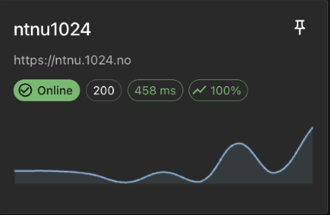
\includegraphics[width=\linewidth]{figures/MVP-dashboard/mvp-card.png}
                \caption{MVP website card}
                \label{fig:mvp_dashboard}
            \end{subfigure}
        \end{minipage}
    }
    \caption{Comparison of website card from prototype to MVP}
    \label{fig:websitecards_comparison}
\end{figure}

\paragraph{Website Details Page}

To address requirement F.8 while preserving the clarity of the main dashboard interface, a dedicated website details page was developed. This page was introduced to prevent visual clutter by relocating in-depth data away from the central dashboard view. Users can access the details page by clicking a website card, which opens a separate view containing historical metrics such as response time and uptime statistics. These metrics are presented in the form of time-series graphs and a chronological list of recorded status checks, enabling users to analyse performance trends over time without compromising the simplicity of the primary interface (\autoref{fig:website_details_mvp}).

\begin{figure}[H]
\centering
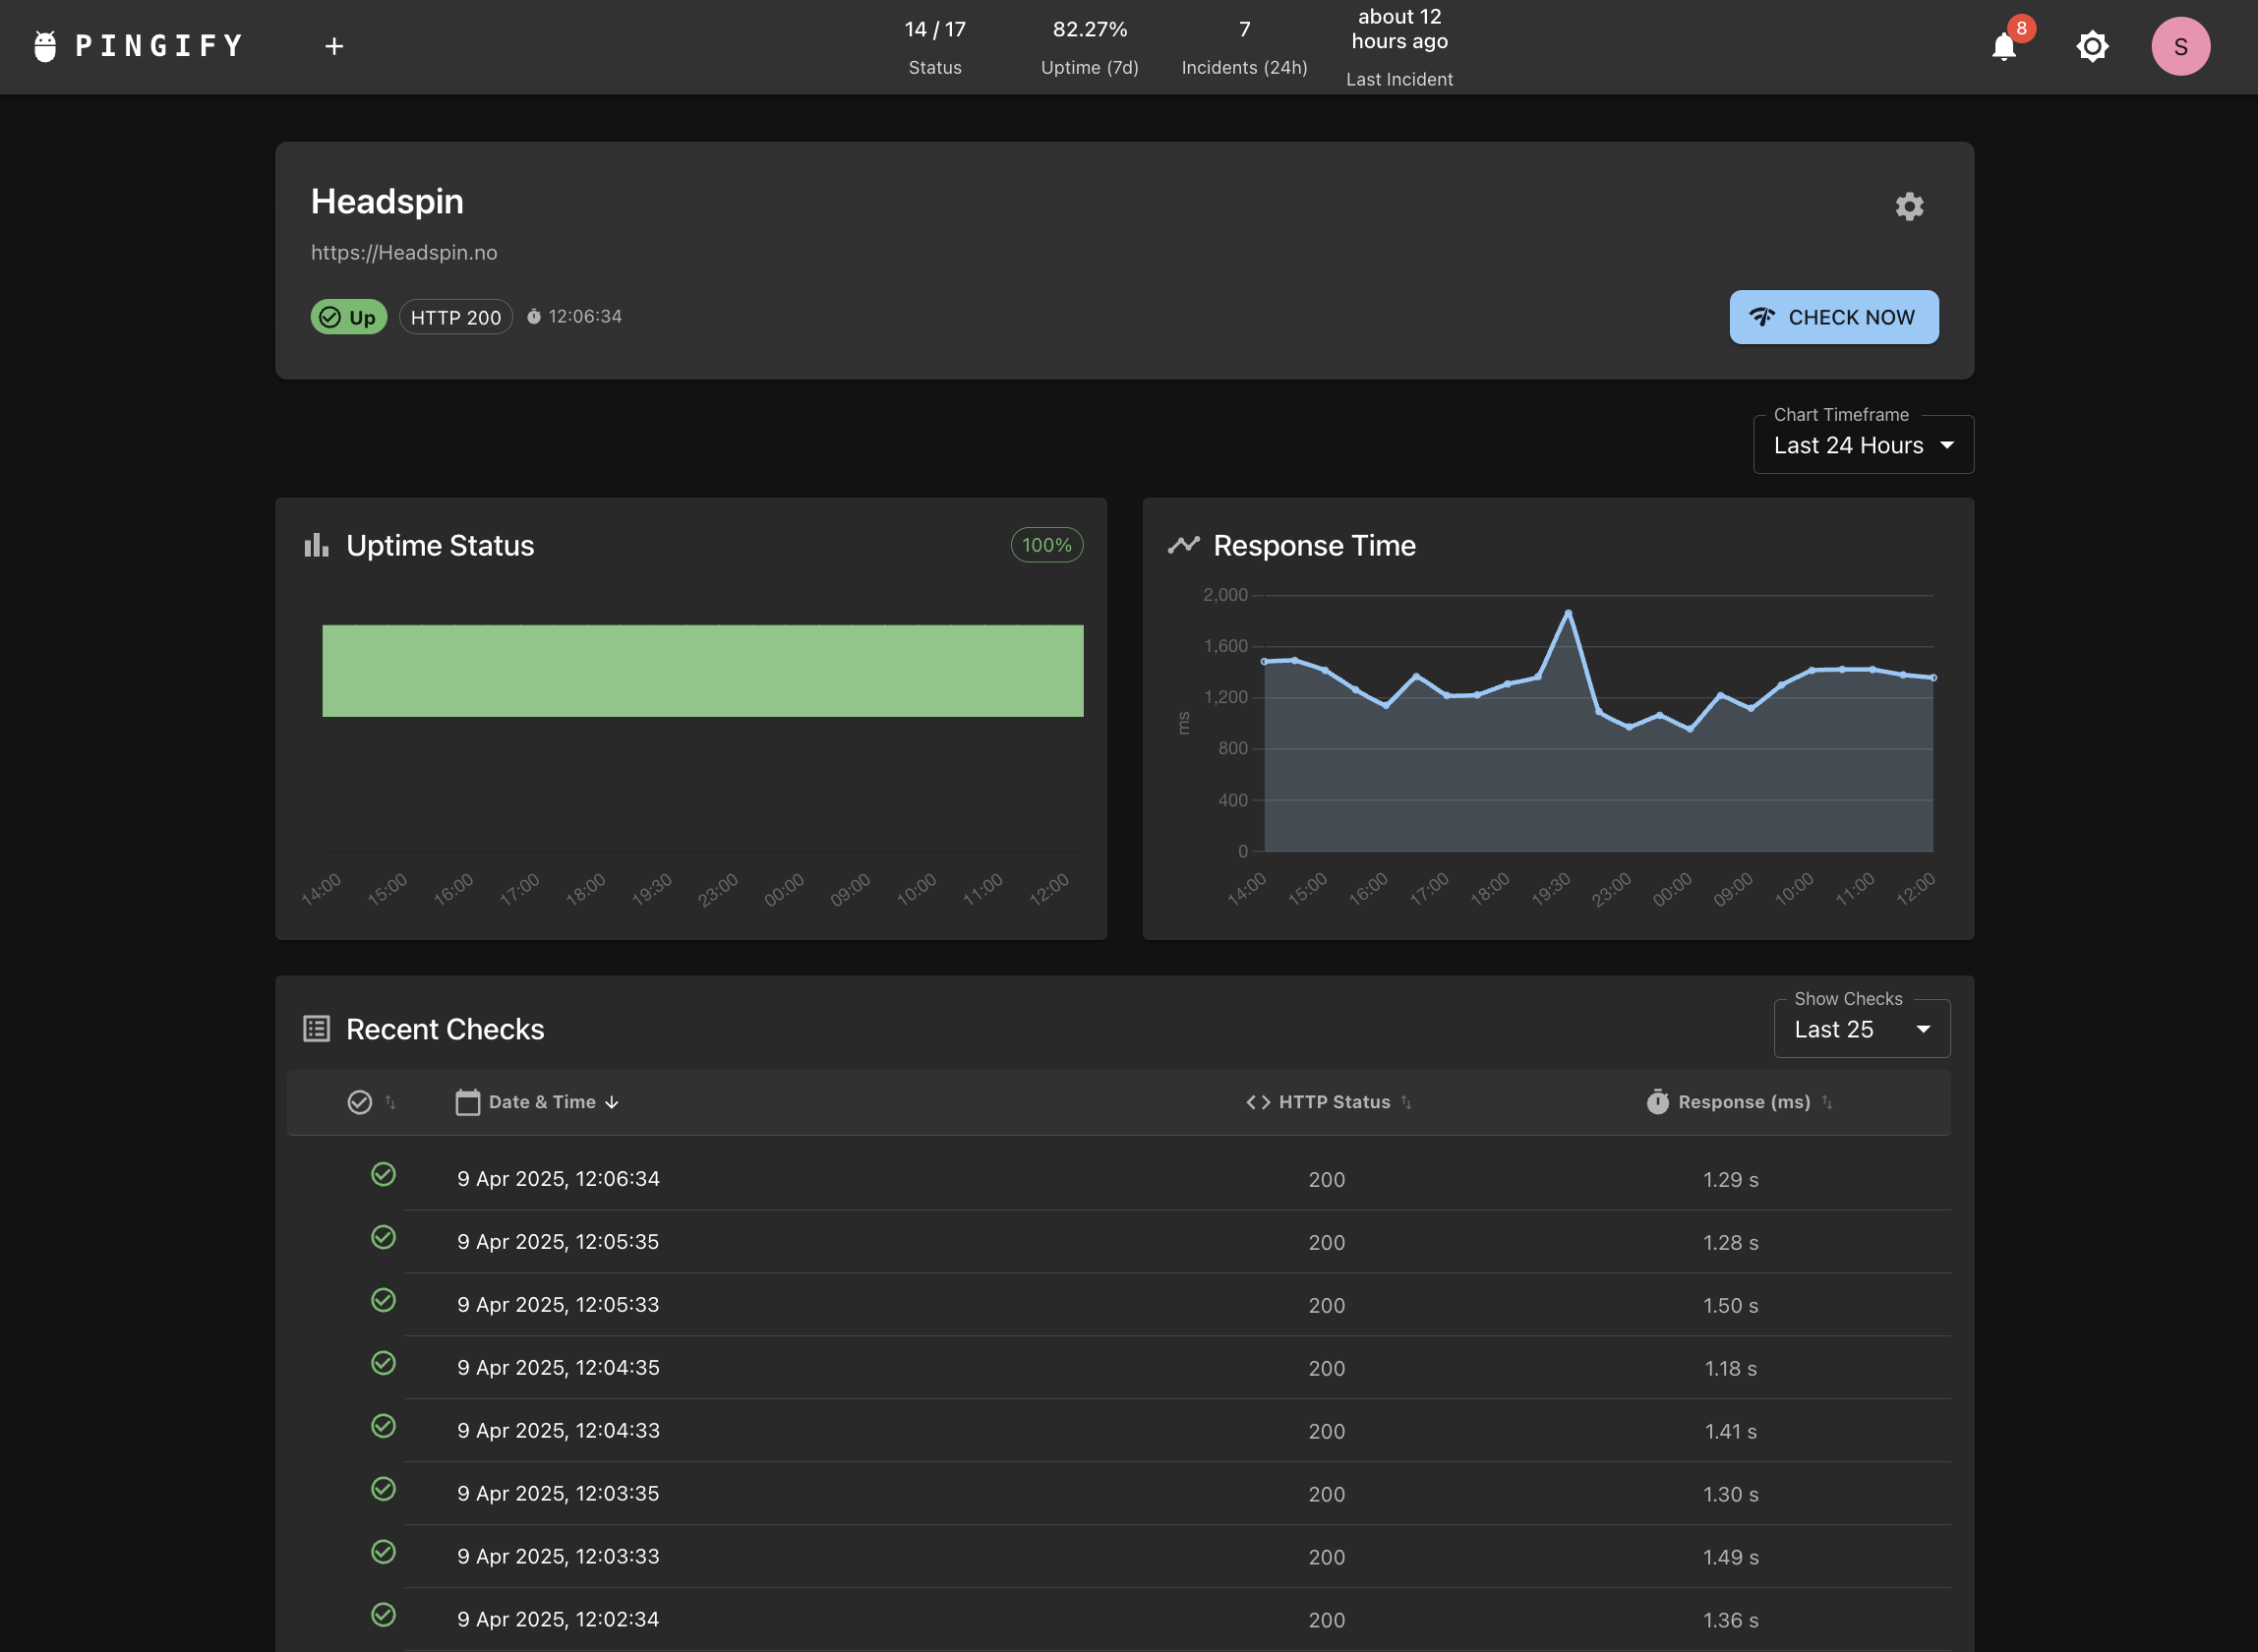
\includegraphics[width=\textwidth]{figures/MVP-dashboard/MVP-websitedetails.png}
\caption{Website details page in the MVP, showing historical uptime and response time data.}
\label{fig:website_details_mvp}
\end{figure}
 
\paragraph{Navigation Bar Redesign}

In response to requirement NF.3, which emphasized the need for a more intuitive and user-friendly interface, the sidebar from the prototype was entirely removed. Its functionality was restructured and integrated into a redesigned top navigation bar, aligning with feedback from P3. The navigation bar consolidates essential controls, including an "Add Website" button positioned adjacent to the logo and access to user settings housed within a drop-down menu under the profile icon. Additional elements, such as a dark/light mode toggle and an alert indicator, were also introduced in the MVP to enhance usability.

To ensure continuous visibility of system status, the navigation bar dynamically displays the current status of all monitored websites when the user is not viewing the main dashboard. Furthermore, filtering and sorting controls for website cards were relocated from the sidebar to the dashboard itself, reinforcing the principle of proximity by placing controls closer to the elements they affect. These changes aimed to streamline user interaction and reduce cognitive load (\autoref{fig:mvp_navbar} , \autoref{fig:mvp_navbar_status}).

\begin{figure}[H]
\centering

\includegraphics[width=1\linewidth]{figures/MVP-dashboard/navbar-mvp.png}
\caption{Navigation bar, with add website button, alert indicator, dark mode toggle, and profile icon}
\label{fig:mvp_navbar}
\end{figure}

\begin{figure}[H]
\centering

\includegraphics[width=1\linewidth]{figures/MVP-dashboard/navbar-mvp-status.png}
\caption{Navigation bar showing general status of the dashboard when the user is not on the main dashboard page}
\label{fig:mvp_navbar_status}
\end{figure}


\paragraph{Navigation Bar Redesign}

In response to requirement NF.3, which emphasized the need for a more intuitive and user-friendly interface, the sidebar from the prototype was entirely removed. Its functionality was restructured and integrated into a redesigned top navigation bar, aligning with feedback from P3. The navigation bar consolidates essential controls, including an "Add Website" button positioned adjacent to the logo and access to user settings housed within a drop-down menu under the profile icon. Additional elements, such as a dark/light mode toggle and an alert indicator, were also introduced in the MVP to enhance usability.

Figure~\ref{fig:mvp_navbar} displays the updated navigation bar as it appears on the main dashboard. The "Add Website" button is placed prominently to the left, followed by the alert indicator and theme toggle. The profile icon on the right grants access to user-specific settings. When users navigate away from the dashboard, the navigation bar adapts to display a condensed status summary, as shown in Figure~\ref{fig:mvp_navbar_status}, maintaining visibility of critical system information.

Furthermore, filtering and sorting controls for website cards were relocated from the sidebar to the dashboard itself, reinforcing the principle of proximity by placing controls closer to the elements they affect. These changes aimed to streamline user interaction and reduce cognitive load.

\begin{figure}[H]
\centering

\includegraphics[width=1\linewidth]{figures/MVP-dashboard/navbar-mvp.png}
\caption{Navigation bar, with add website button, alert indicator, dark mode toggle, and profile icon}
\label{fig:mvp_navbar}
\end{figure}

\begin{figure}[H]
\centering

\includegraphics[width=1\linewidth]{figures/MVP-dashboard/navbar-mvp-status.png}
\caption{Navigation bar showing general status of the dashboard when the user is not on the main dashboard page}
\label{fig:mvp_navbar_status}
\end{figure}

\paragraph{Status Banner}

To fulfil requirement F.9, which called for an overview of system-wide status information, a status banner was introduced at the top of the dashboard interface. This component displays key summary metrics, including the number of websites currently operational or down, the overall uptime percentage across all monitored websites, the number of incidents reported within the last 24 hours, and the time since the most recent incident happened.

As illustrated in \autoref{fig:mvp_status_bar}, the banner is positioned above the website cards and is displayed alongside other interface components such as the search bar, filtering options, and the focus mode toggle (explained in next section).

\begin{figure}[H]
\centering
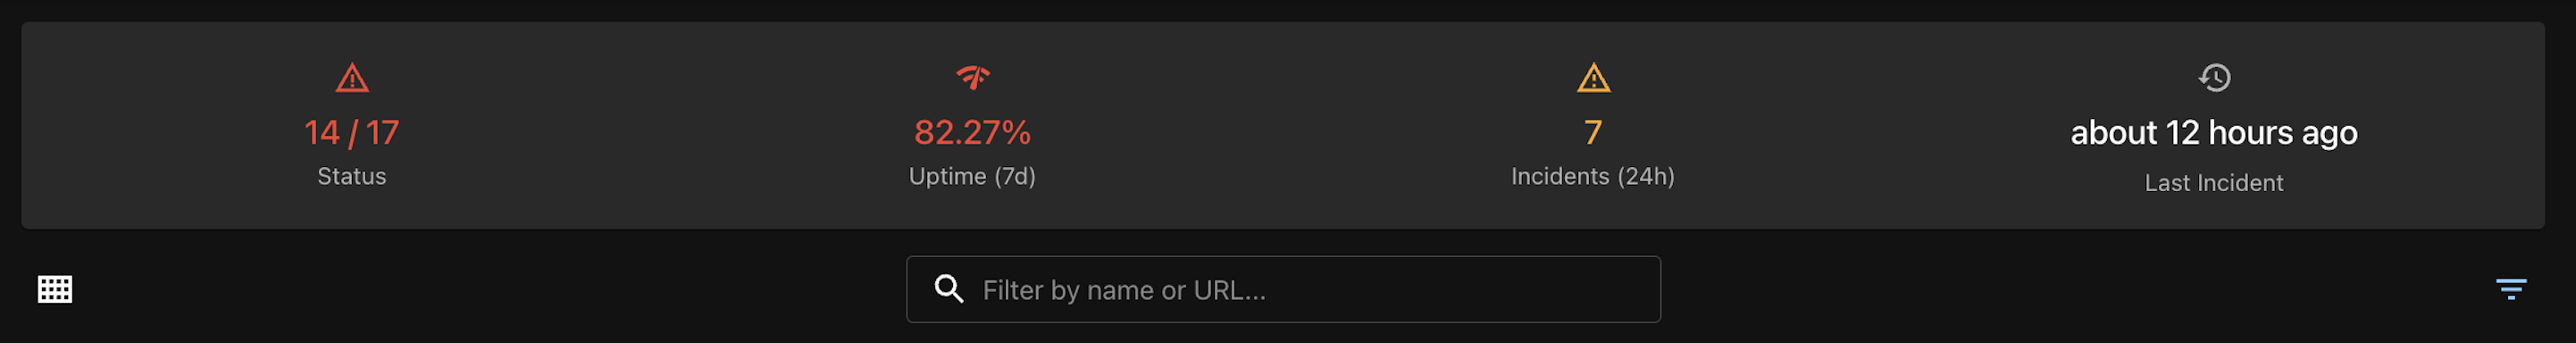
\includegraphics[width=0.8\linewidth]{figures/MVP-dashboard/MVP-statusbanner.png}
\caption{Status banner with "focus mode", search bar, and filter-button}
\label{fig:mvp_status_bar}
\end{figure}



\paragraph{Focus Mode}
Focus mode was introduced in response to informal feedback from Headspin indicating that the dashboard could be displayed on large screens around the office. No requirement for a focus mode was elicited, meaning that we developed this feature on our own initiative ahead of user test 2. Focus mode was designed to showcase as many monitored websites as possible without cluttering the interface or requiring user interaction. Pressing the "focus mode" icon, as seen in \autoref{fig:mvp_focus_mode}, makes the status banner and navigation bar hidden, giving more space on the screen to website cards cards, making them more prominent and easier to for the user to scan at a glance. The focus mode indirectly addresses NF.2, by making website status changes easy to see at a glance. Focus mode was renamed to tv mode, and further improved after user test 2.

\begin{figure}[H]
    \centering
    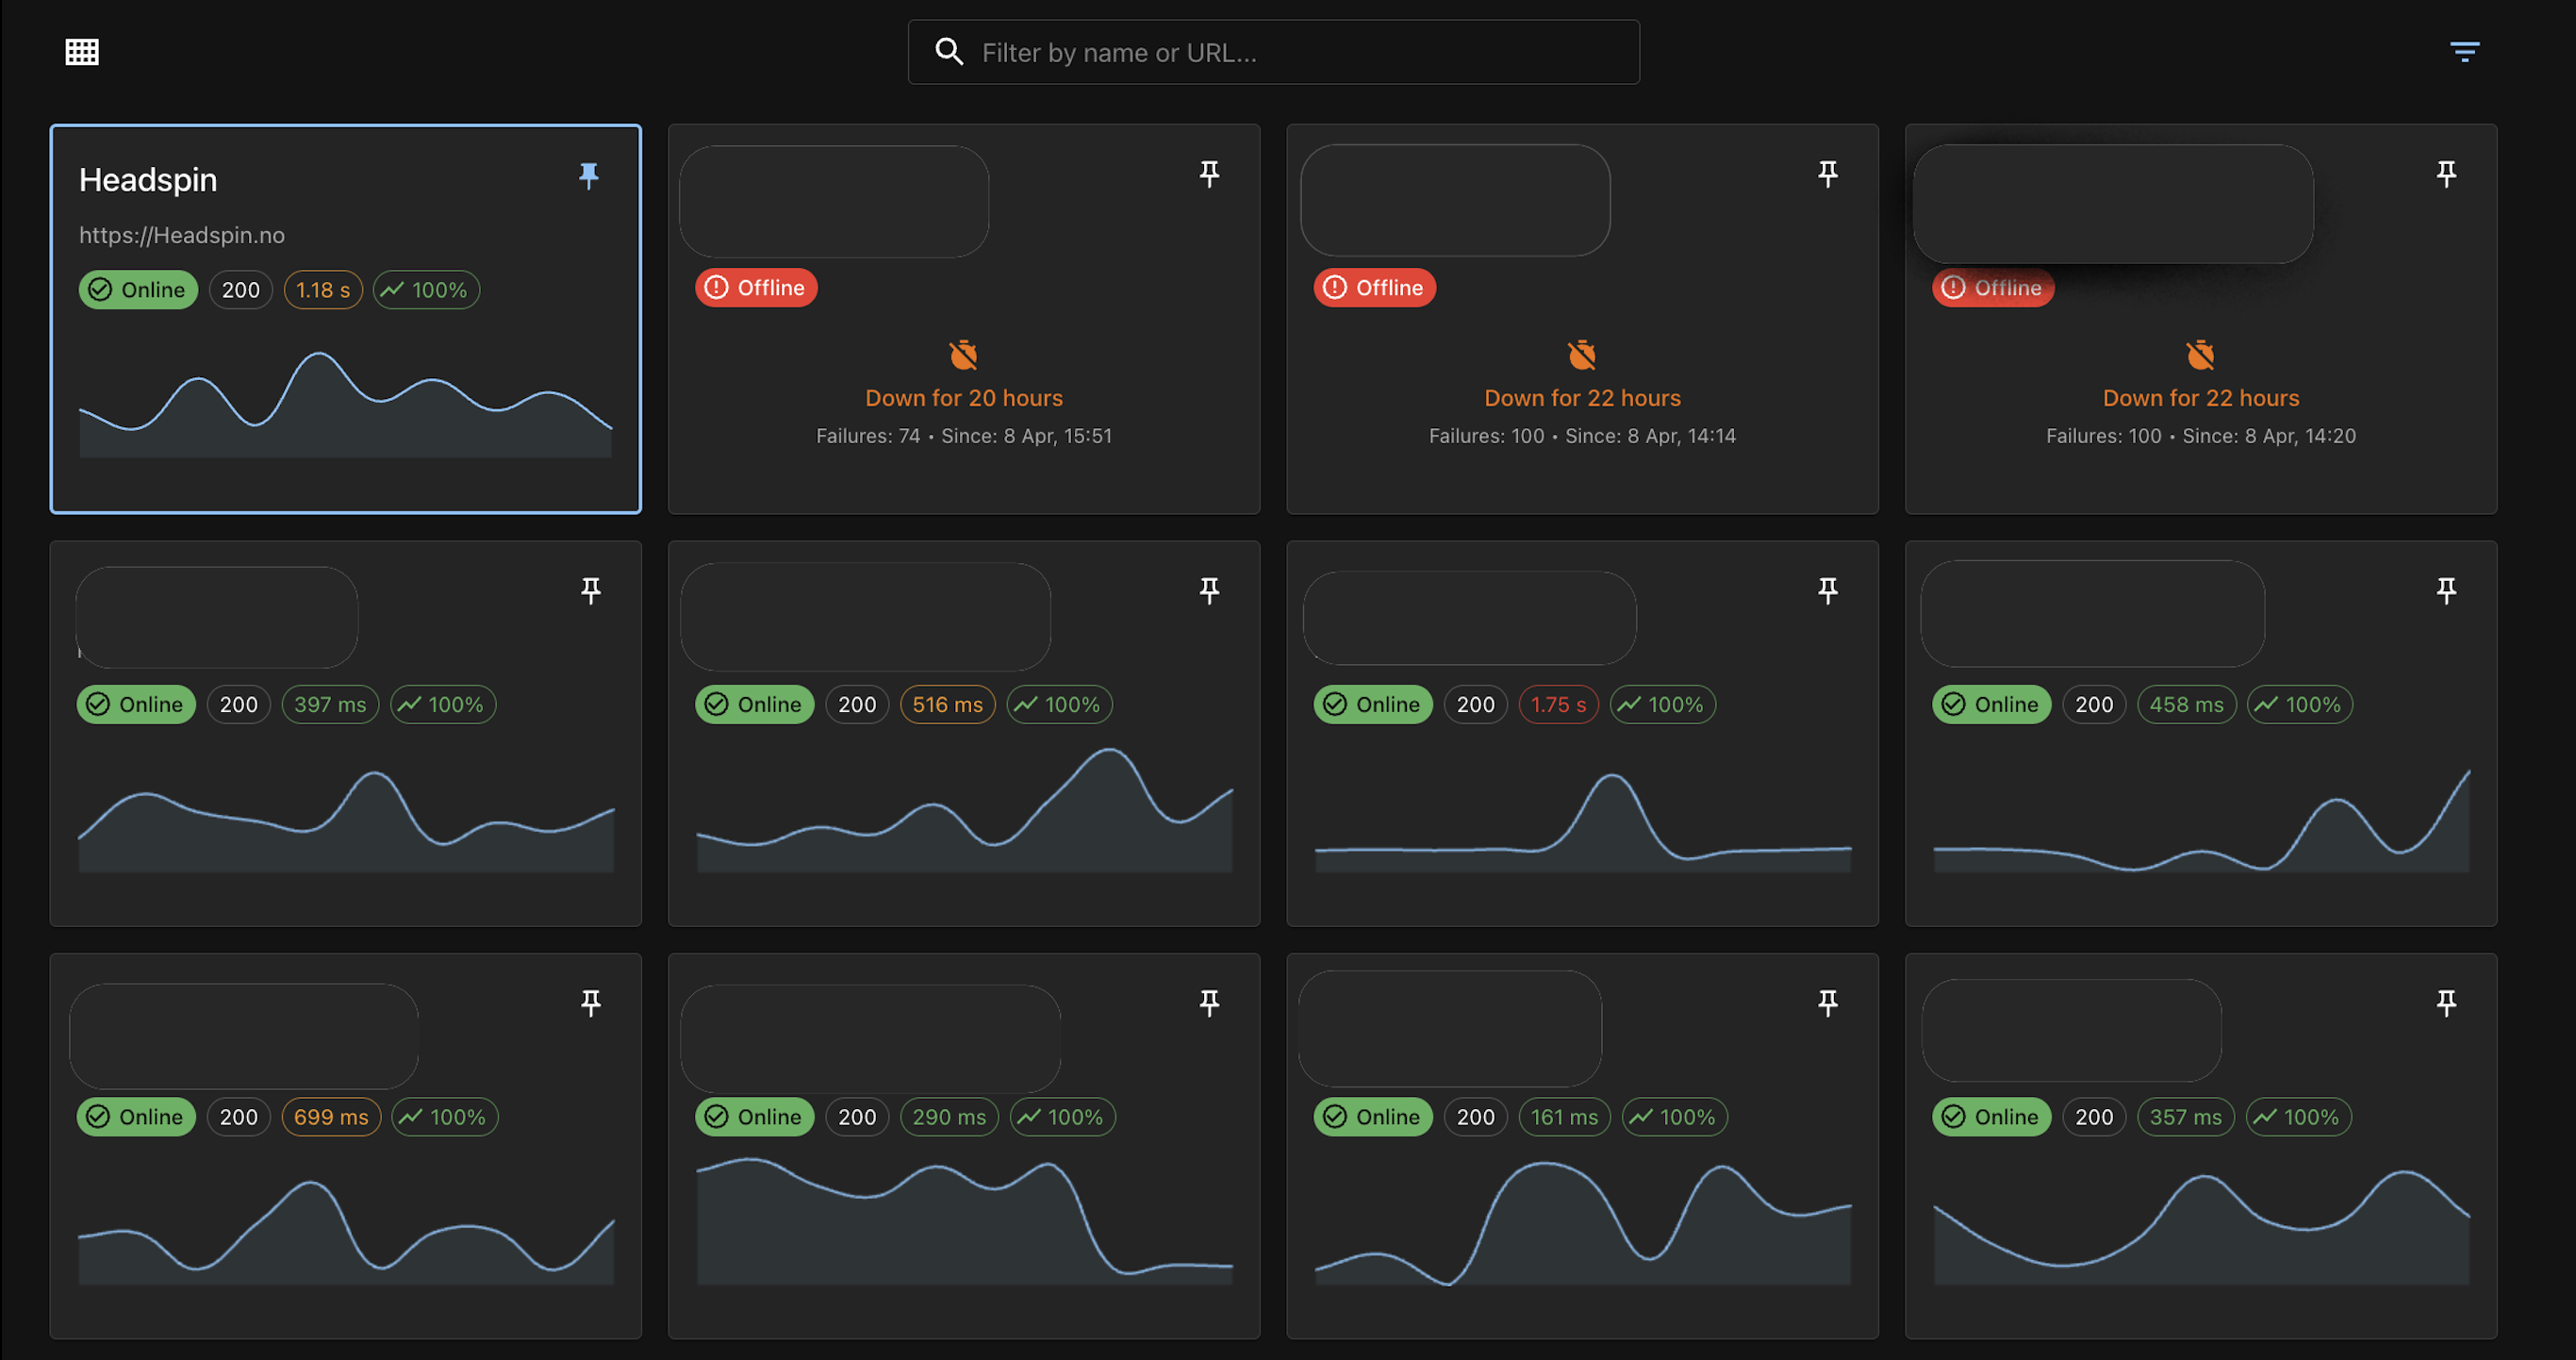
\includegraphics[width=0.8\linewidth]{figures/MVP-dashboard/MVP-focus-mode.png}
    \caption{Focus mode}
    \label{fig:mvp_focus_mode}
\end{figure}

\paragraph{Focus Mode}

Focus Mode was introduced based on informal feedback from Headspin, which indicated that the dashboard might be displayed on large screens in shared office spaces. Although this feature was not part of the original requirements specification, it was proactively developed ahead of user test 2 to support passive monitoring in such environments.

Focus Mode is activated via a dedicated icon on the dashboard. Once enabled, the navigation bar and status banner are hidden, maximizing the screen real estate allocated to the website cards. This design makes the the dashboard cards more visually prominent and reduces interface distractions. As shown in \autoref{fig:mvp_focus_mode}, the focus mode layout  facilitates being able to monitor status of website at a glance, and indirectly supports requirement NF.2 by improving the clarity of status information. The feature was renamed to TV Mode following user test 2, during which further enhancements were made to its visual presentation.

\begin{figure}[H]
\centering
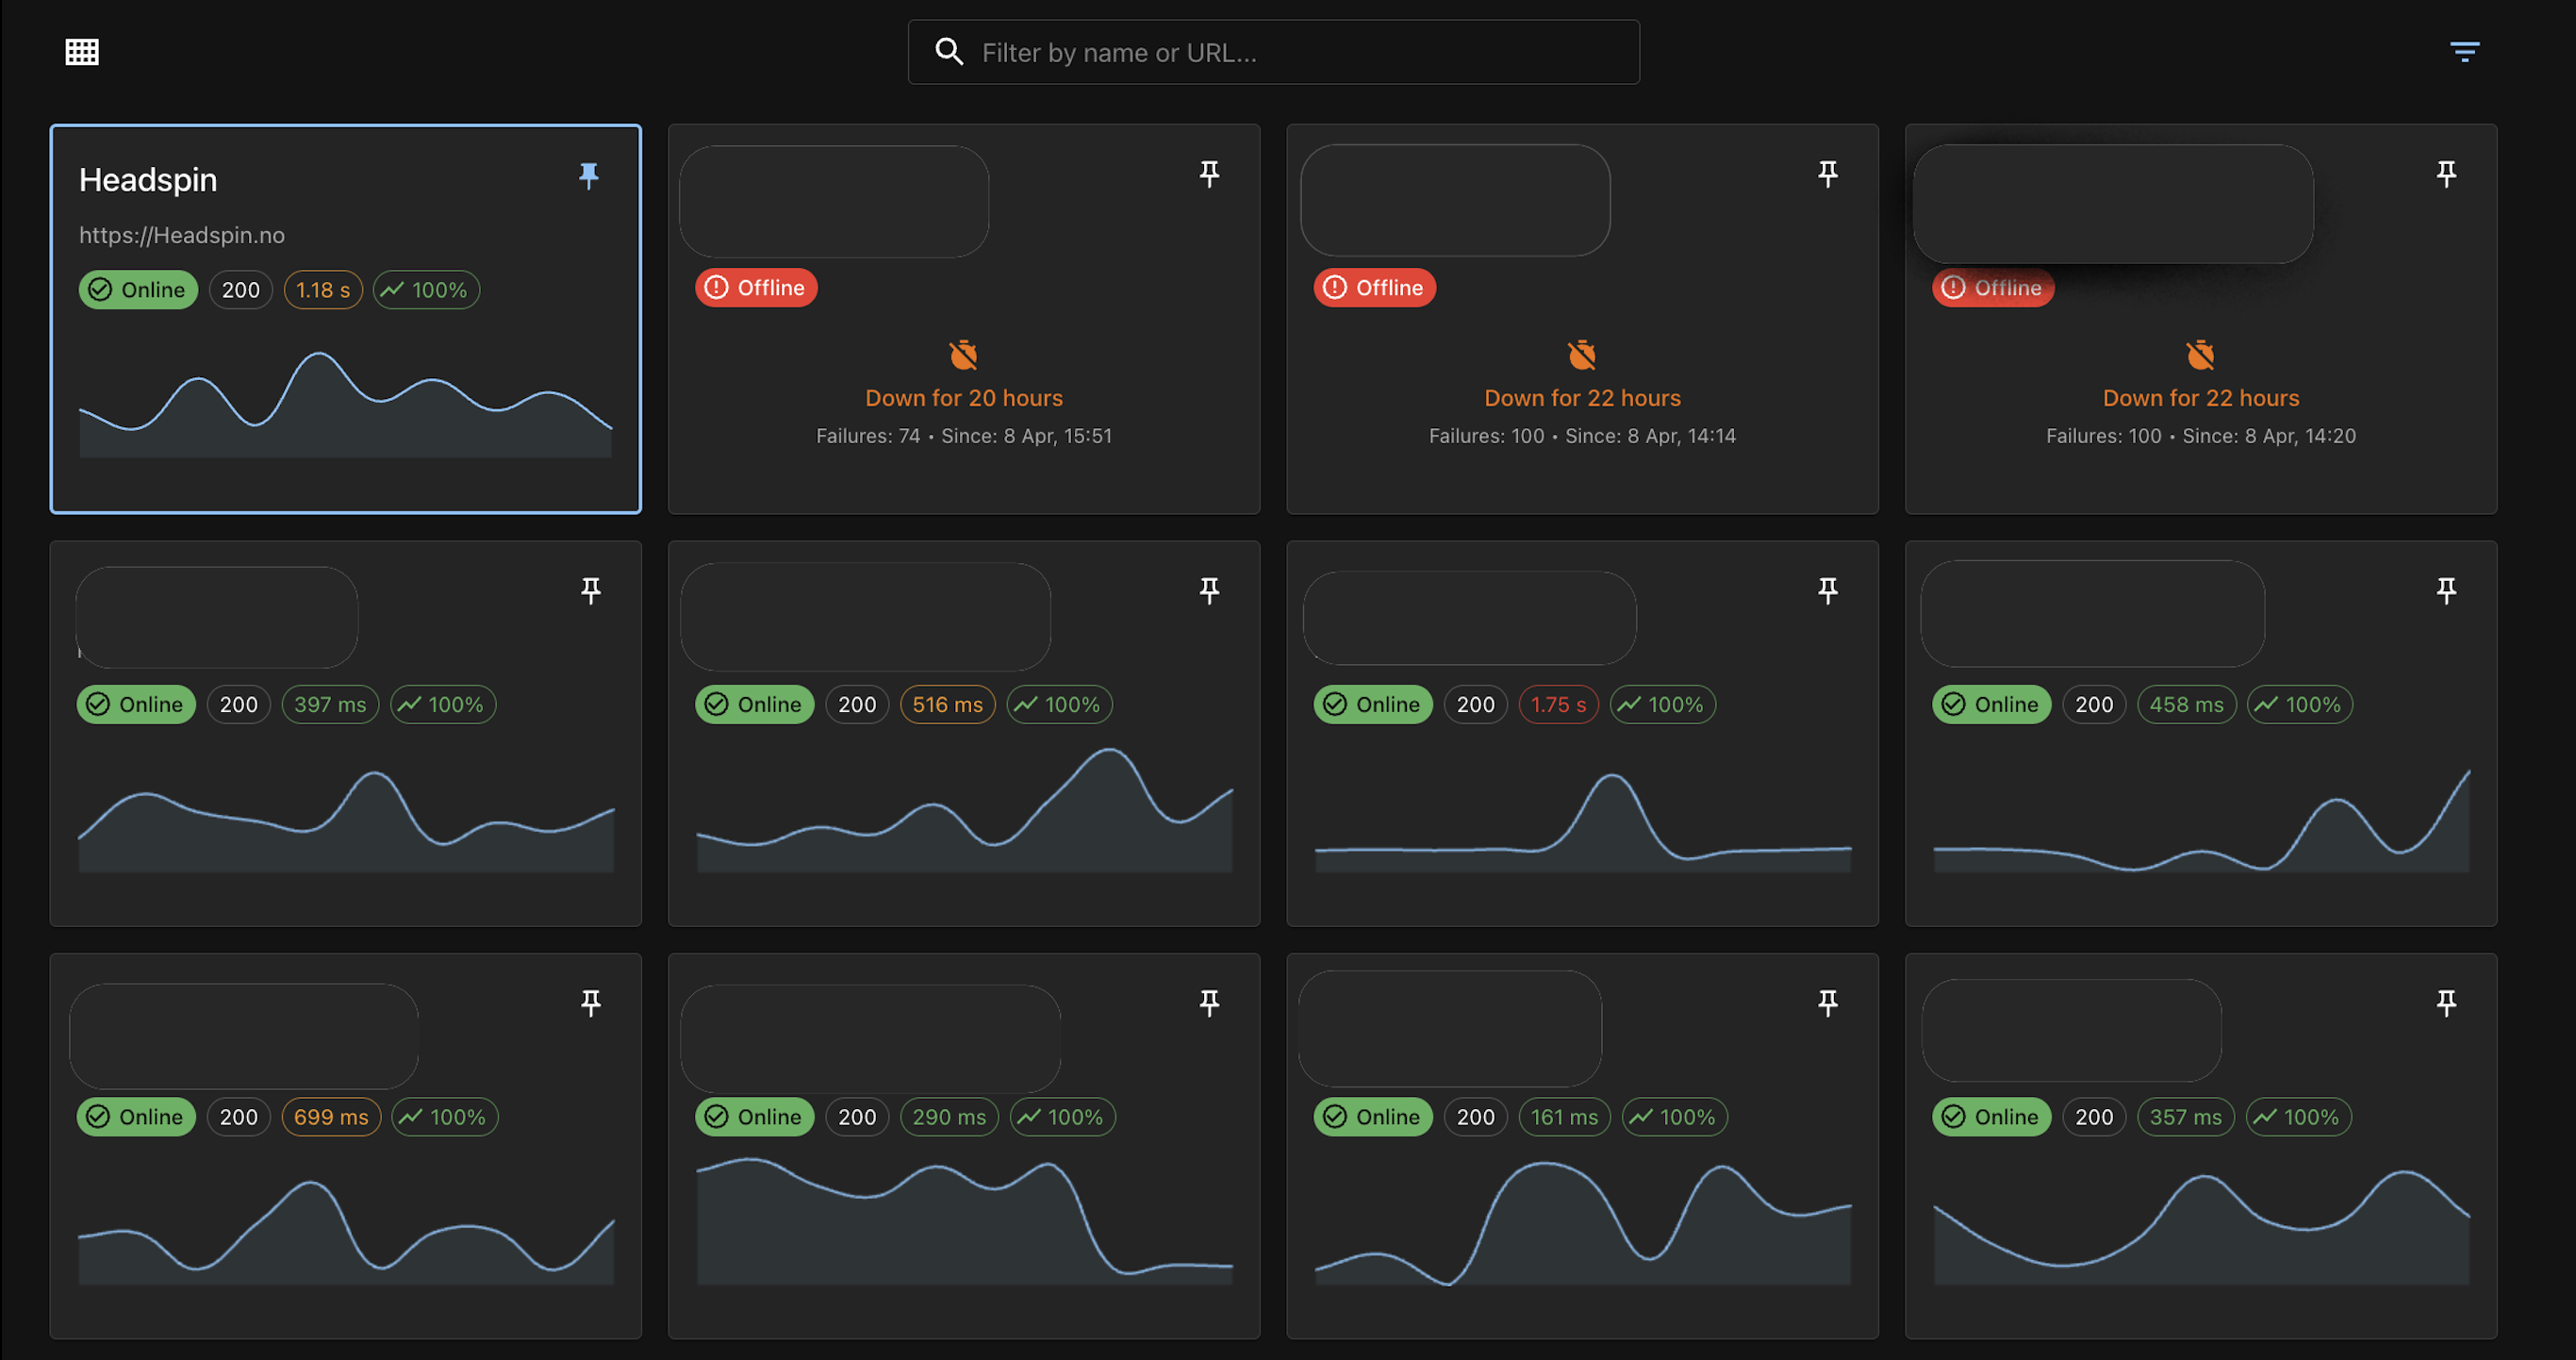
\includegraphics[width=0.8\linewidth]{figures/MVP-dashboard/MVP-focus-mode.png}
\caption{Focus Mode view, with navigation and status elements hidden to prioritize status card visibility}
\label{fig:mvp_focus_mode}
\end{figure}

\paragraph{Filtering}
Filtering functionality was implemented in the form of a drop-down menu and a search bar. The filter menu allows the user to filter website cards alphabetically or by response time, as seen in \autoref{fig:final_filtering_button}, while the search bar enables searching by user defined website name, or URL.

\begin{figure}[H]
    \centering
    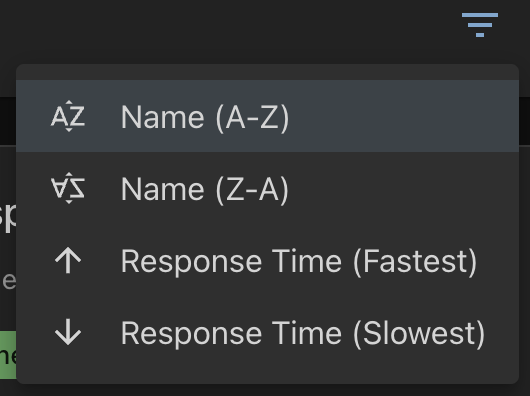
\includegraphics[width=0.5\linewidth]{figures/final_application/final-filteringbutton.png}
    \caption{Filtering icon with open filtering menu}
    \label{fig:final_filtering_button}
\end{figure}

\paragraph{Filtering}

To support efficient navigation and content management on the dashboard, filtering functionality was implemented through a combination of a drop-down menu and a search bar. The drop-down menu enables users to filter website cards based on alphabetical order or response time, allowing them to quickly prioritize or locate relevant information.

As shown in \autoref{fig:final_filtering_button}, the filtering icon opens a compact menu that offers multiple sorting options. Complementing this, the search bar supports free-text input based on user-defined website names or URLs, further enhancing usability for dashboards containing numerous monitored websites. These filtering mechanisms were designed in alignment with interface usability heuristics that emphasize visibility of system status and user control.

\begin{figure}[H]
\centering
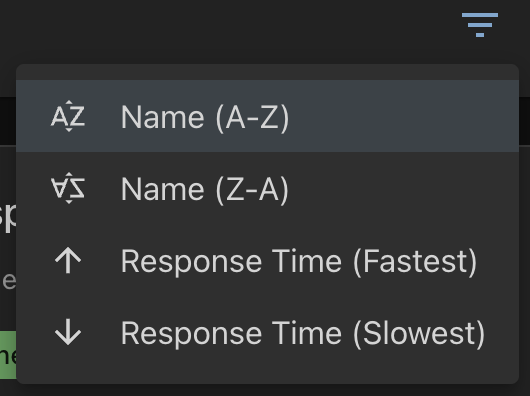
\includegraphics[width=0.5\linewidth]{figures/final_application/final-filteringbutton.png}
\caption{Filtering icon with open filtering menu}
\label{fig:final_filtering_button}
\end{figure}

%%%%%FORTSETT MED CHATTING HER IMORGEN FRED ER IK
\paragraph{User Authentication}
User authentication  was implemented to support user login, registration, and personalized dashboards, responding to requirement F6. This functionality users to manage their own set of websites in the dashboard application. When logged in, alerts, and website with custom names are private to each user. Users can also set dark or light mode, which is saved indefinitely. Figure~\ref{fig:login_page} displays how users log in to use the dashboard.

\begin{figure}[H]
    \centering
    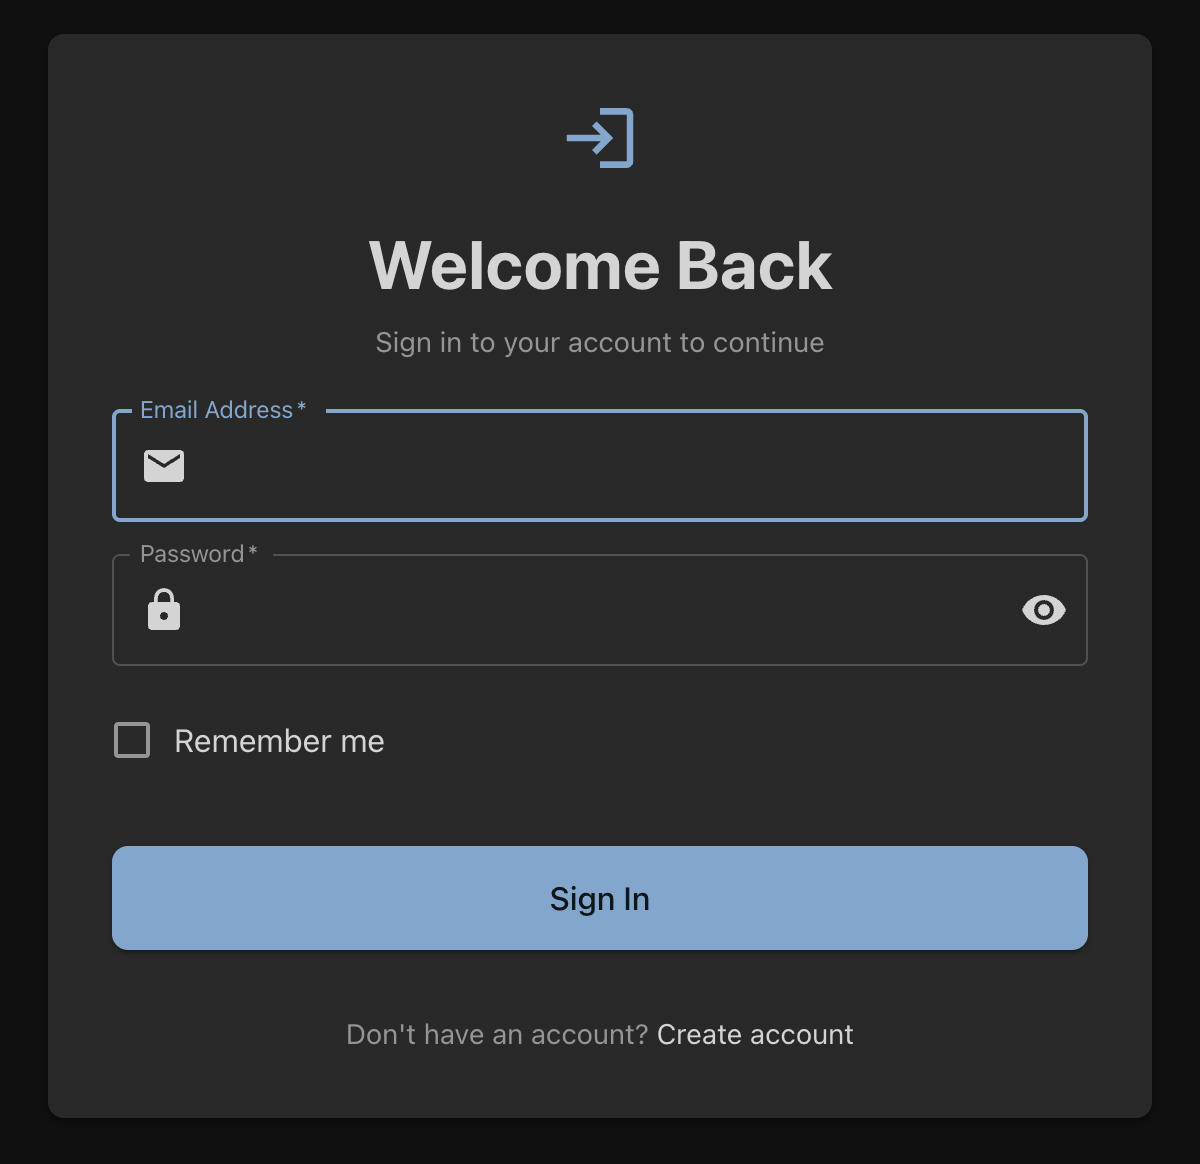
\includegraphics[width=0.6\linewidth]{figures/final_application/final_loginpage.png}
    \caption{Login Page}
    \label{fig:login_page}
\end{figure}

\paragraph{Pinning}
One of these features is pinning. This adheres to requirements F.10 and F.6 and allows users to mark specific websites as important. Pinning a website card automatically moves it to the top of the dashboard, as seen in Figure~\ref{fig:mvp_pinned_card} (also seen in Figure~\ref{fig:mvp_dashboard}).

\begin{figure}[H]
    \centering
    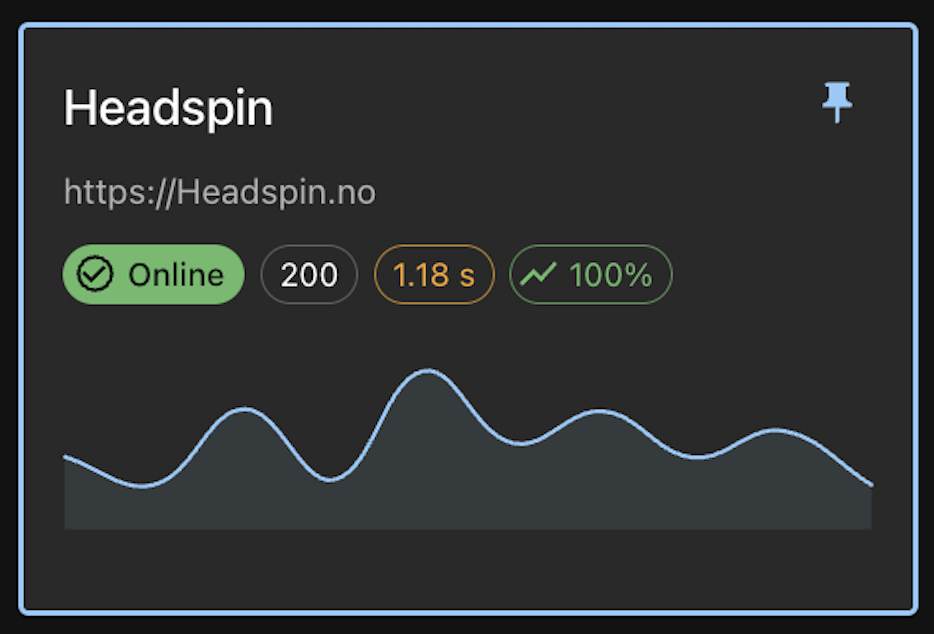
\includegraphics[width=0.5\linewidth]{figures/MVP-dashboard/MVP-pinned-card.png}
    \caption{Pinned Website Card}
    \label{fig:mvp_pinned_card}
\end{figure}

\paragraph{Alert System}
The system's monitoring logic was implemented using \texttt{\gls{axios}} for \gls{http} requests and the \texttt{\gls{cron}} module to trigger status checks at user-defined intervals, directly addressing F.2. If a check resulted in a website being down, or the response time being slower than the user-defined interval, a new check was triggered to confirm the original result. If the result was confirmed, an incident was created, and an alert was triggered. Users can define thresholds for acceptable response times, and alerts are dispatched only when these defined constraints are violated. Clicking on the alert icon in the navigation bar opens a list of triggered alerts, as illustrated in Figure~\ref{fig:alertlist}

\begin{figure}[H]
    \centering
    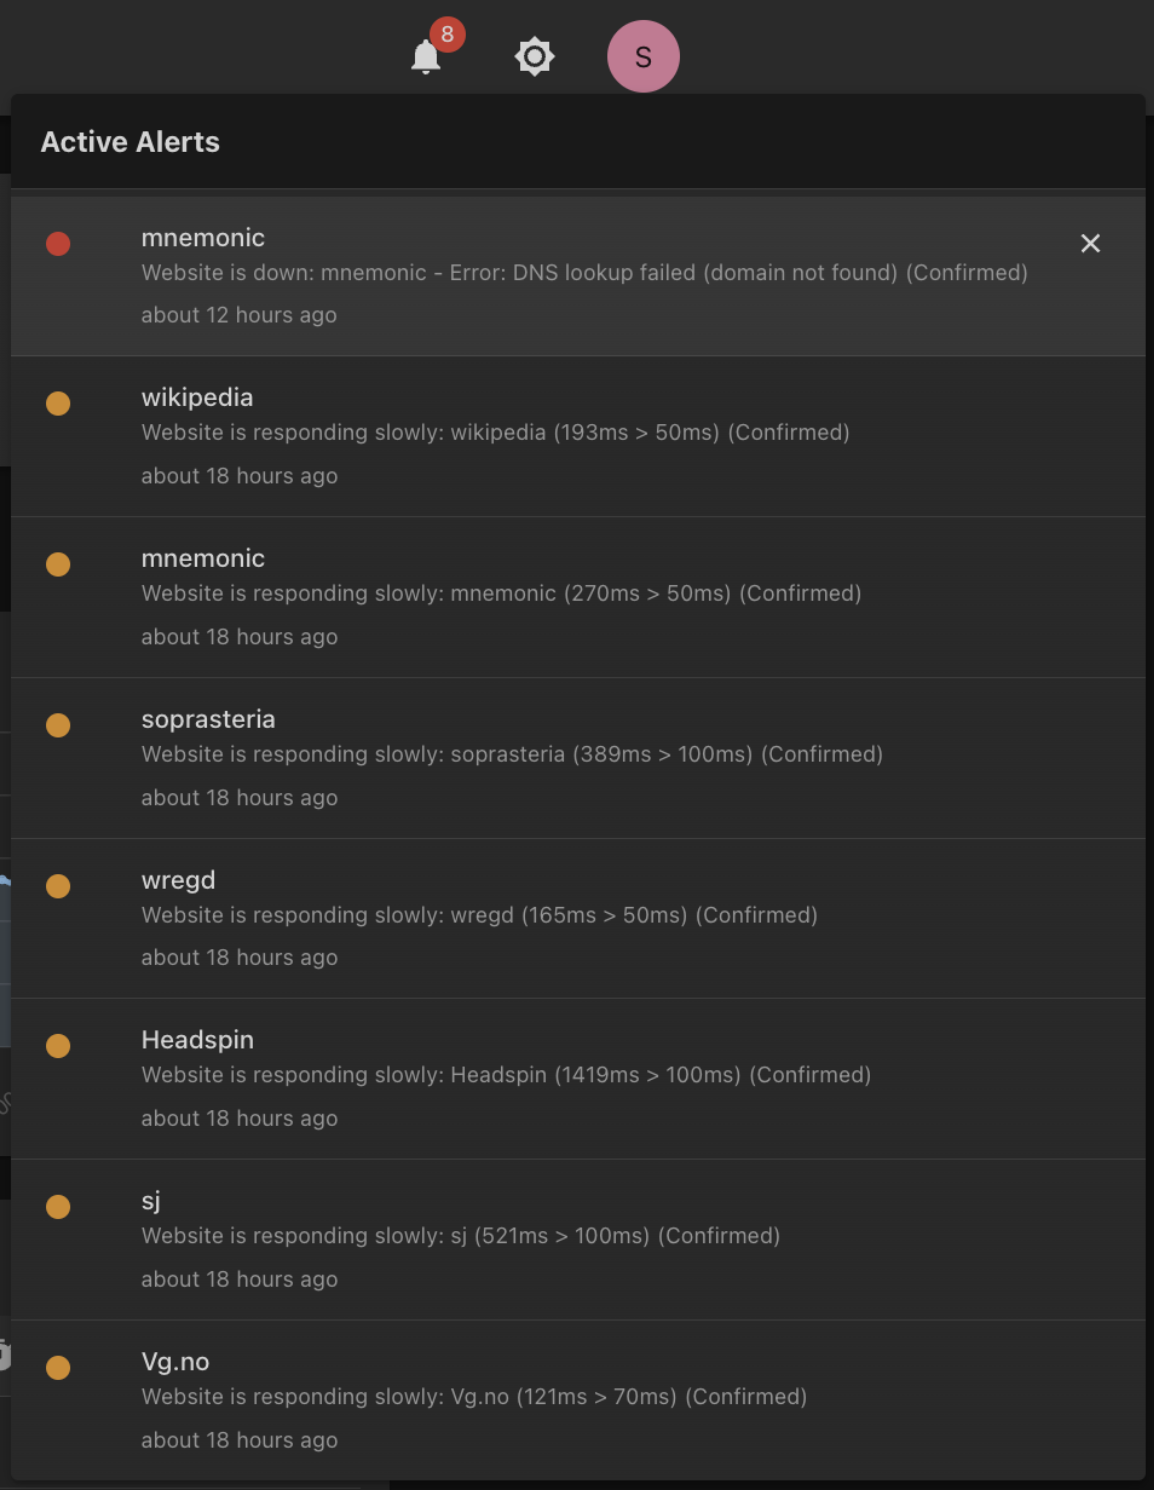
\includegraphics[width=0.65\linewidth]{figures/MVP-dashboard/MVP-only_alertlist.png}
    \caption{List with example alerts}
    \label{fig:alertlist}
\end{figure}

As seen in Figure~\ref{fig:mvpaddwebsite}, adding a new website enables users to configure custom check intervals, per F.2, and have the option to enable alerts. Alert settings included defining a response time threshold and specifying a notification email address, fulfilling requirement F.5. 

\begin{figure}[H]
    \centering
    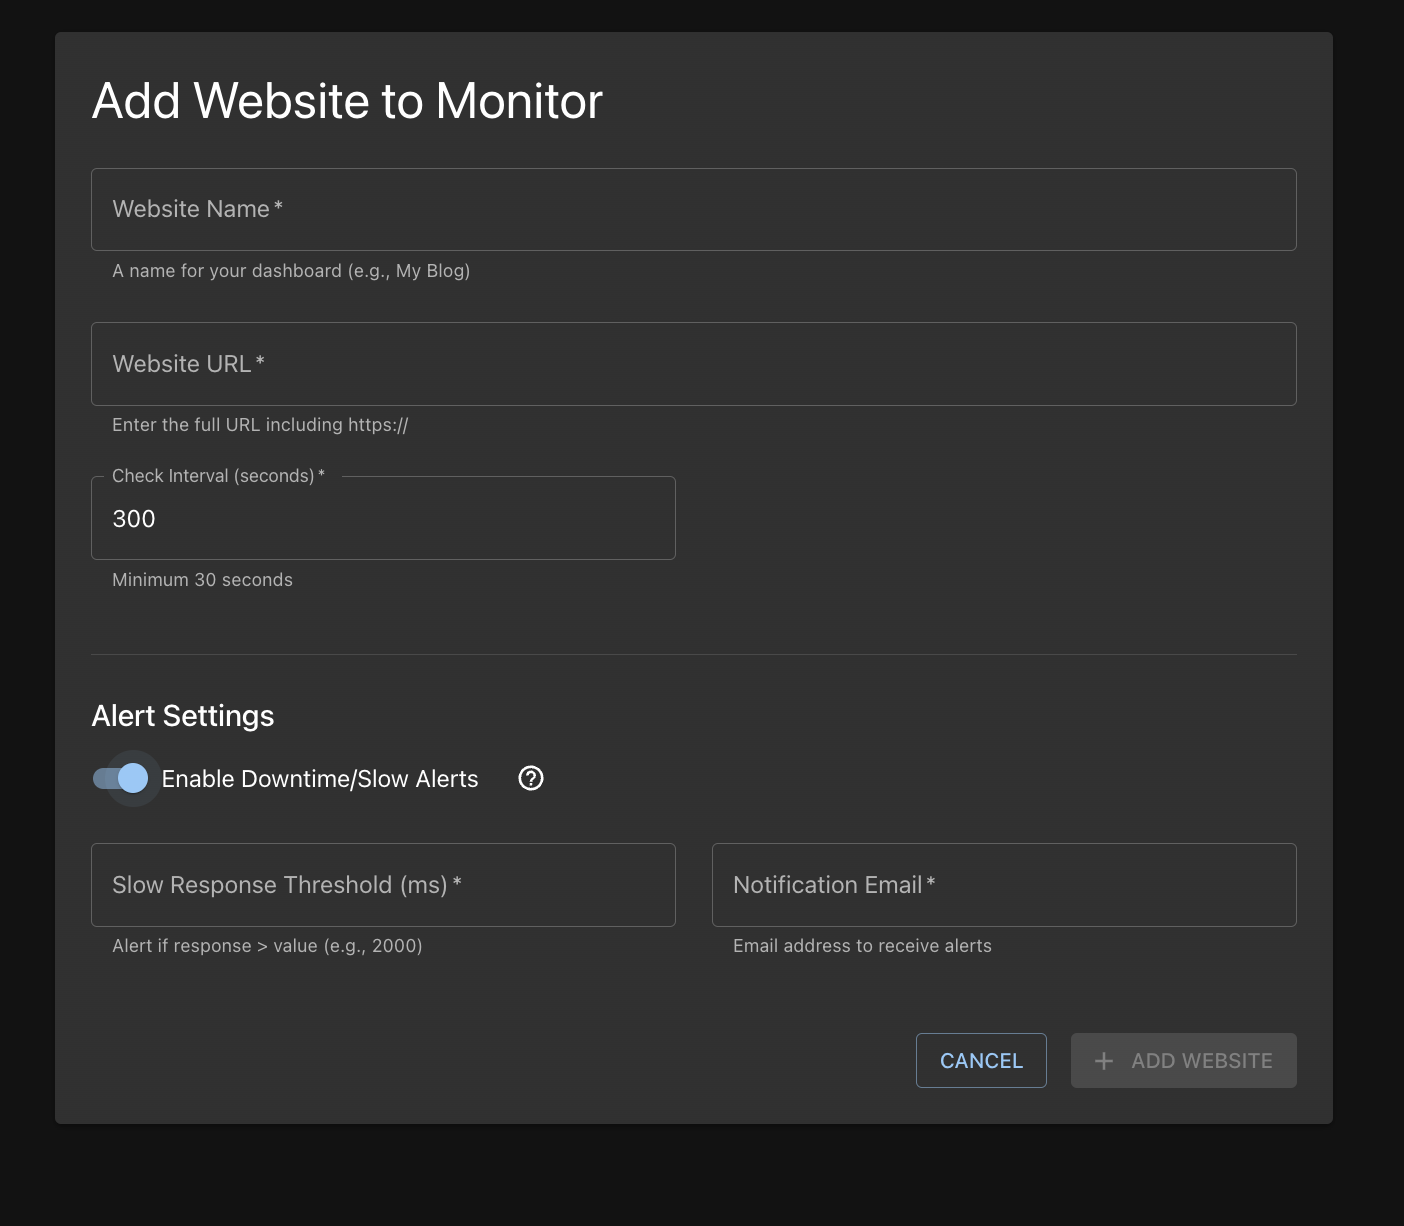
\includegraphics[width=0.6\linewidth]{figures/MVP-dashboard/MVP-addwebsite.png}
    \caption{Options when adding a new website}
    \label{fig:mvpaddwebsite}
\end{figure}



\subsubsection{Feedback from MVP (User Test 2)}  
No participants had any objections to the presentation of the new dashboard cards with the updated status indicators, and changed background colours. However, some new usability issues emerged. All three participants raised confusion about the values represented in the response time graphs on the dashboard cards. P1 commented that the graph lacked a title, legend, and time axis, making it difficult to interpret. This feedback led to the creation of requirement F.11, seen in \autoref{tab:req_usertest_2}

P1 also noted that the downtime (left) graph in the newly added website details page (\autoref{fig:website_details_mvp}),  should be clickable in order to navigate to a view where the user can see what caused the graph to turn red. P2 also suggested that the graph needed clearer colour coding and scaling to represent issue severity.  In addition to verbal feedback, P2 attempted to click on the downtime graph legend, expecting interactivity, indicating a mismatch between user expectations and actual functionality, supporting P1's statement. P1 noted there was a lack of details and a general overview of incidents. This led to requirement F.12 being created.

Most of the issues regarding navigation were resolved after user test 1, with the addition of the new navigation bar, however two new issues regarding navigation were raised in user test 2. P2 still expressed the need for a more intuitive and central way to add new websites, and P3 spent much time figuring out how to return to the dashboard from the Website Details page, noting the absence of a visible "go back" button. Both address a lack of intuitiveness of the layout, requirement NF.3. 

We also received feedback from P1, regarding the new status banner, which stated that it took up to much vertical space on the dashboard, that could be used to fit more website cards instead, addressing the already existing requirement NF.2, with system status not being displayed clearly. 

%requireemnts direkte fra MVP user test 2
\begin{table}
    \centering
    \begin{tabular}{|c|p{0.72\linewidth}|c|} \hline
    \textbf{ID} & \textbf{Requirement Description} & \textbf{Priority} \\ \hline
         F.11&  Graphs on cards needs title, legend, and time axis& Medium\\ \hline 
         F.12&  Incident tracking system with incident list& High\\\hline
    \end{tabular}
    \caption{Additional Functional and Non-Functional requirements from user test 2}
    \label{tab:req_usertest_2}
\end{table}


Following the second round of user testing, the focus shifted to addressing newly discovered usability issues and refining existing features. While the updated dashboard cards and status indicators were positively received, participants identified several areas needing improvement. Key areas included data visualization, navigation, and spatial layout. These insights informed the final development phase before project hand-off.

\subsubsection{Implementing Feedback from User Test 2}

\paragraph{Incident System}
In the \acrshort{MVP}, incidents were only displayed within the dashboard's status banner (\autoref{fig:statusbar}). Incidents were generated solely based on alerts. Consequently, if a user had disabled alerts for a particular website, no incident would be created even if the website experienced downtime or response time degradation. Furthermore, dismissing an alert would result in the corresponding incident being removed, regardless of whether the underlying issue had been resolved. Feedback from user test 2 identified this behaviour as both confusing and inadequate, particularly in terms of communicating ongoing issues. As a result, requirement F.12 was formulated.

To address these limitations, the incident system was redesigned and expanded, to rely on periodic website status checks that are persistently stored in the \gls{database}. This change ensured that incidents are now created independently of user-defined alert settings and are not removed upon alert dismissal. Instead, an incident is marked as resolved only when the system, through regular status checks, detects that the condition that triggered the incident has been rectified. For instance, an incident caused by a website outage is marked as resolved once the system detects that the website is accessible again. Similarly, an incident due to high response time is resolved when the response time improves and falls below the user-defined alert threshold. Alerts are now triggered only if the user has explicitly enabled them for the website in question, while incidents are tracked regardless.

The revised system introduces multiple points of visibility for incidents. A dedicated incident page was developed to provide users with an overview of all incidents, both active and resolved, across the websites associated with their dashboard (\autoref{fig:incident_list}). This page includes filtering options based on incident type and time frame. The dashboard’s status banner (\autoref{fig:statusbar}), unchanged from the MVP, continues to display the number of incidents that have occurred in the past 24 hours, along with the time elapsed since the most recent incident. Additionally, a new banner was added to the website details page to highlight ongoing incidents for individual websites, thereby improving visibility when users navigate away from the main dashboard (\autoref{fig:details_incident_banner}). To further enhance usability, the system automatically reorders dashboard cards to prioritize websites with active incidents, placing those experiencing downtime above those with performance issues.



\begin{figure}[H]
\centering
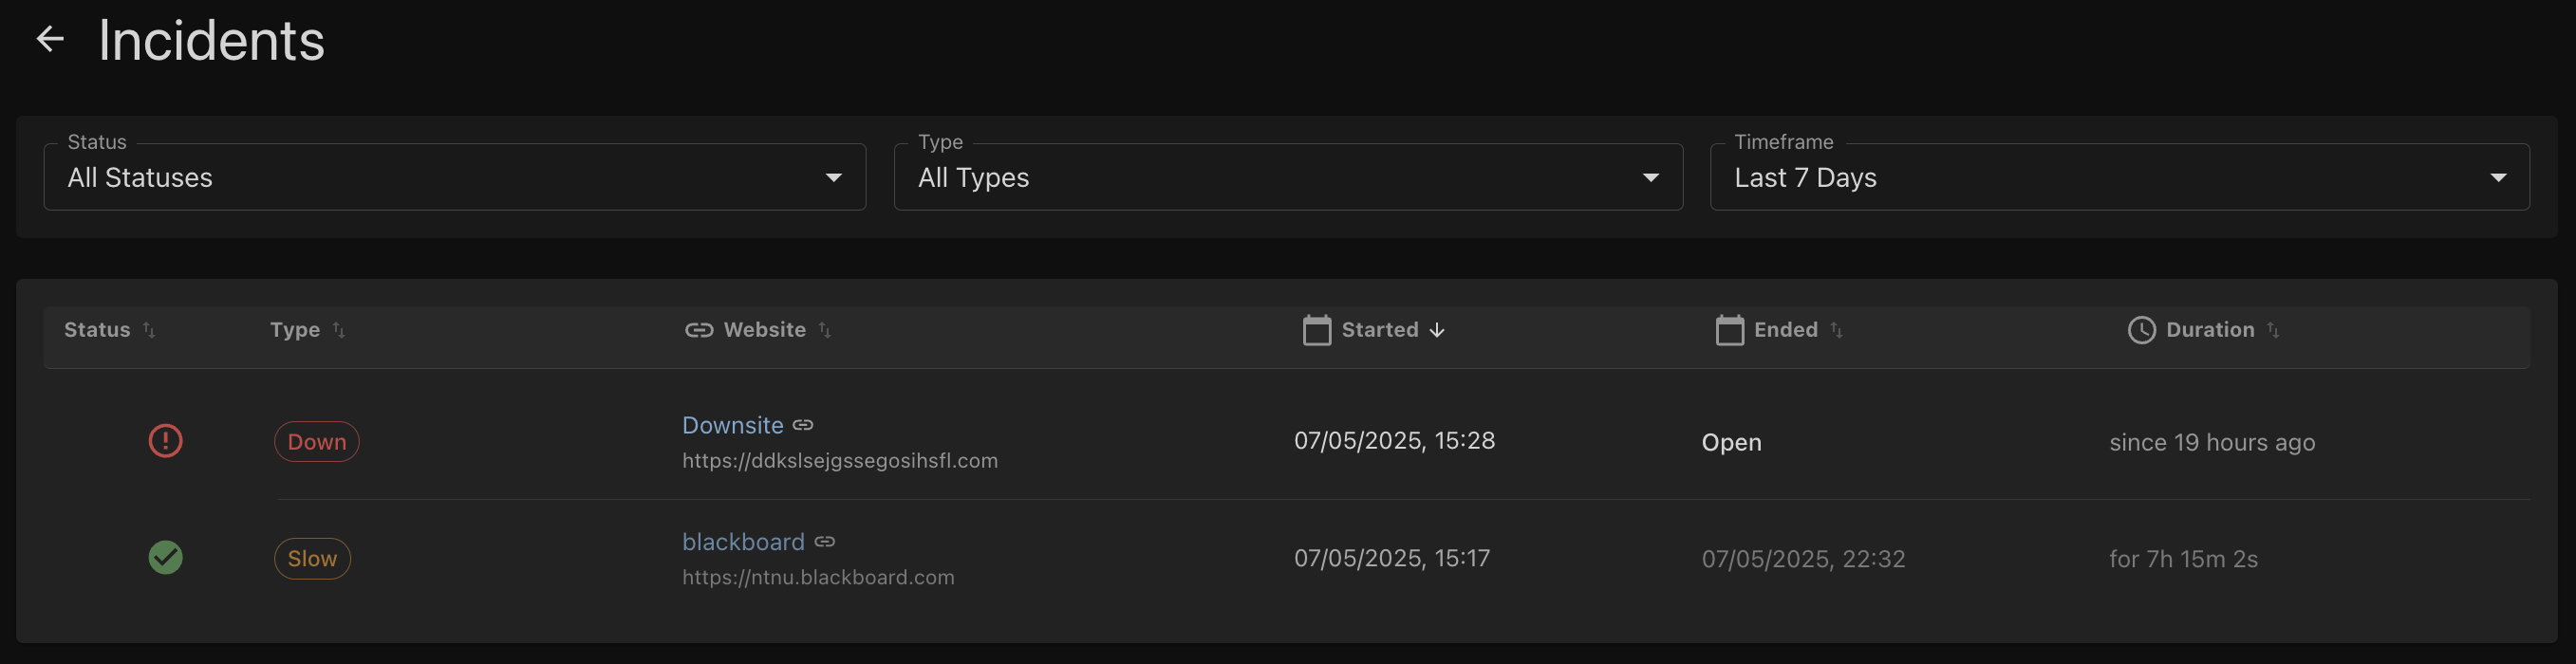
\includegraphics[width=1\textwidth]{figures/IncidentList.png}
\caption{Incident list, showing one ongoing "down" incident, and one resolved "slow"}
\label{fig:incident_list}
\end{figure}

\begin{figure}[H]
\centering
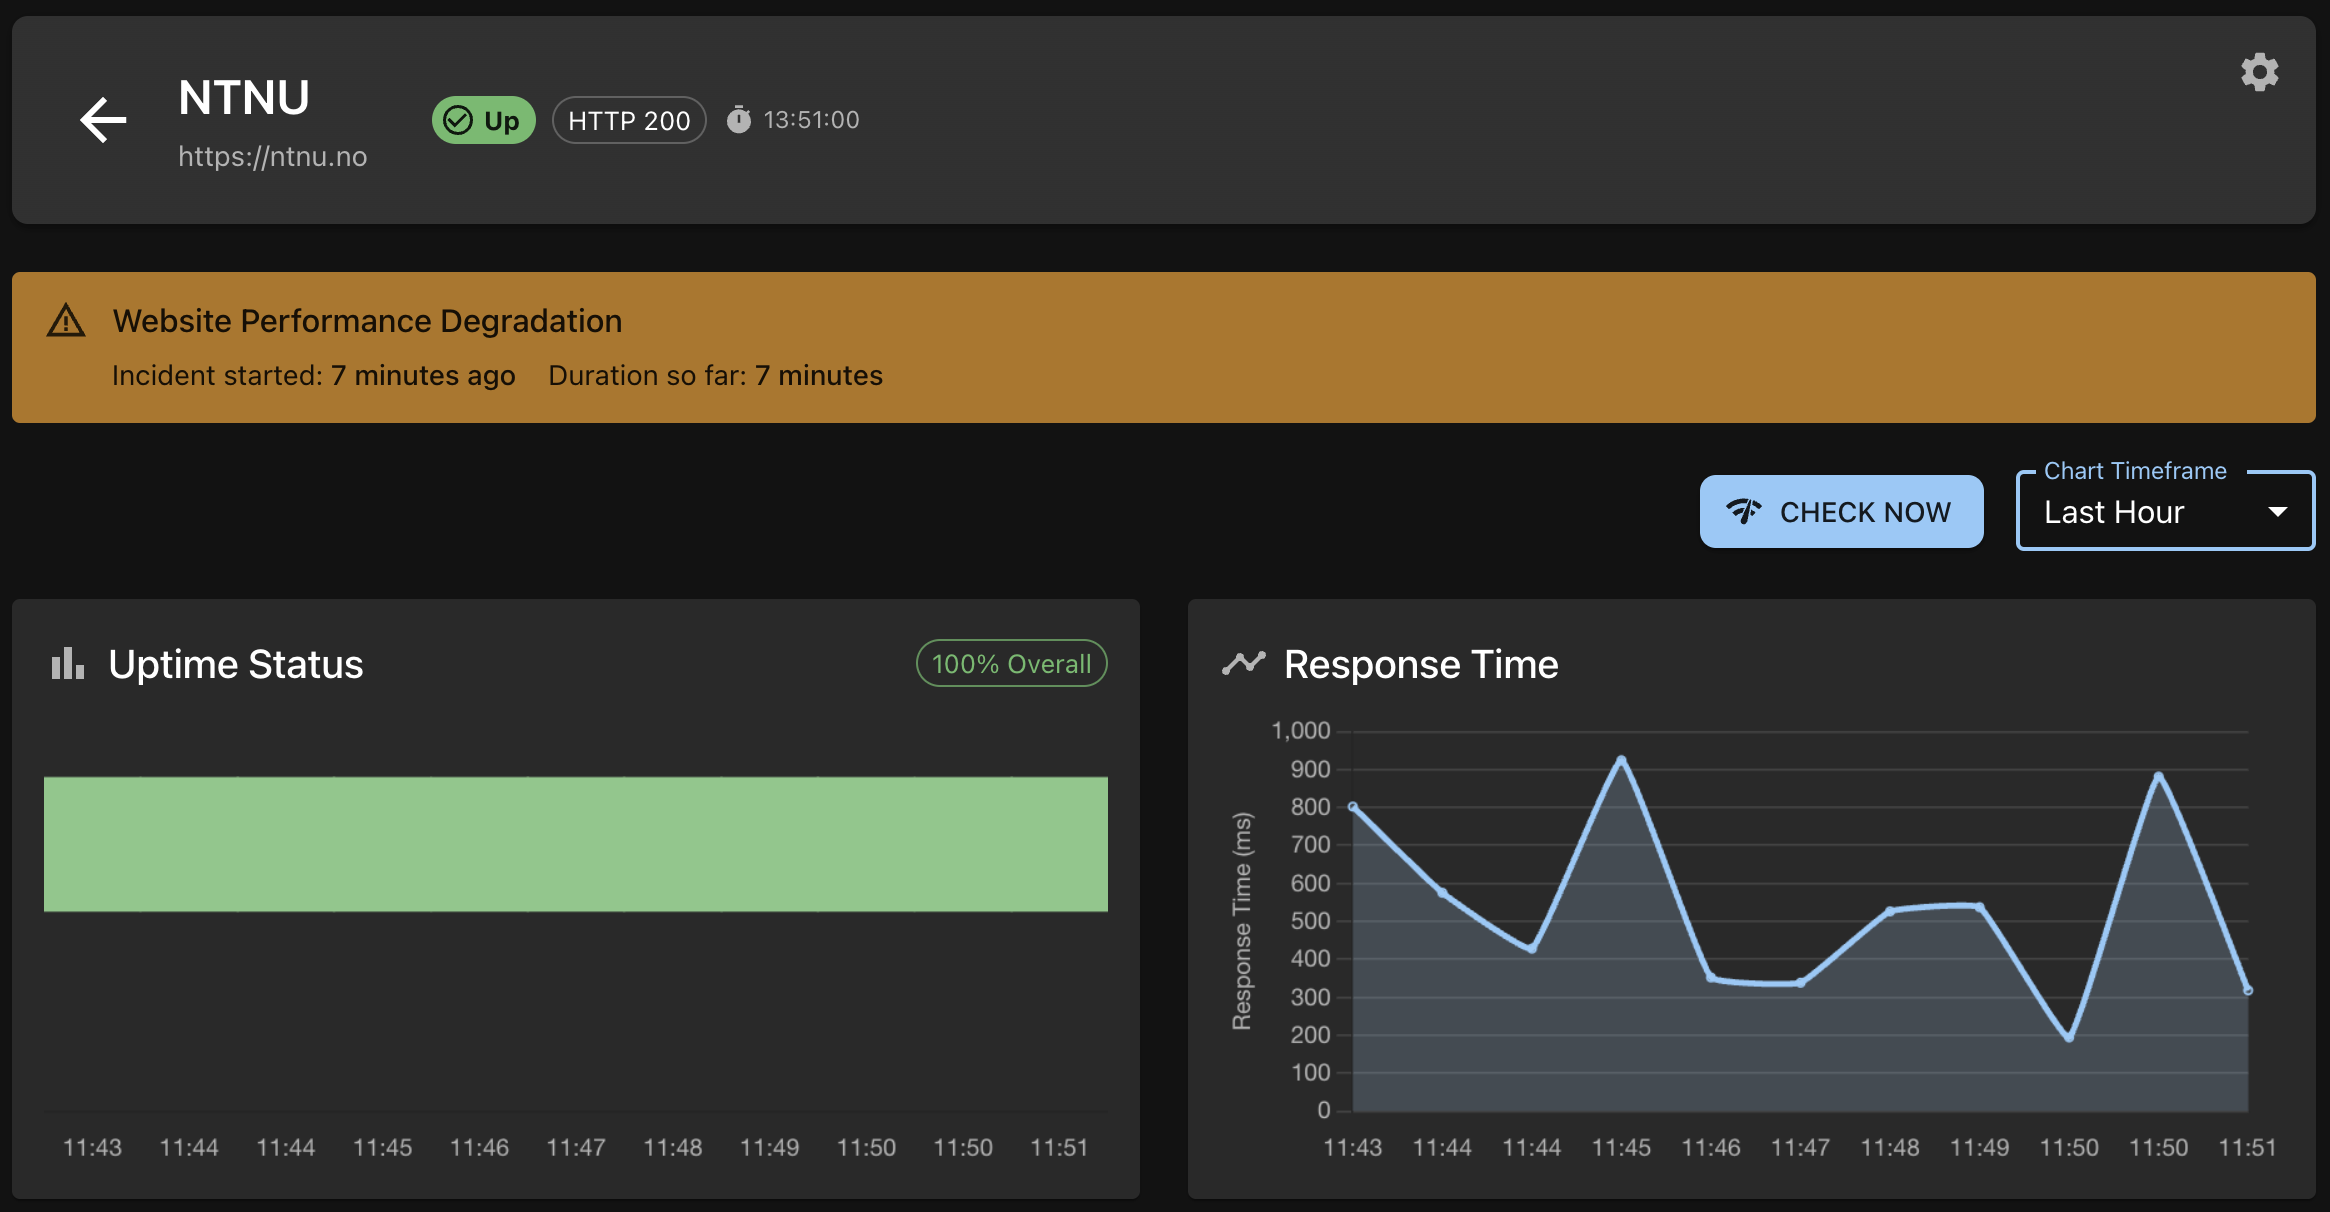
\includegraphics[width=1\textwidth]{figures/websiteDetails.png}
\caption{Banner showing ongoing "slow" incident on website details page}
\label{fig:details_incident_banner}
\end{figure}



\paragraph{Card Graphs with Tooltip}
Although the visual presentation of the dashboard cards was well received, all three participants expressed confusion over the response time graphs. In response to requirement F.11, to support the meaning of the data point in the original graph, a supporting graph representing historical uptime was implemented. In addition, the data points of the original graph got a hover feature, which displays a tooltip, meaning that when a user moves the cursor above a specific data point, a descriptive text pops up. These changes can be seen in Figure~\ref{header_websitedetails}.
\begin{figure}[H]
    \centering
    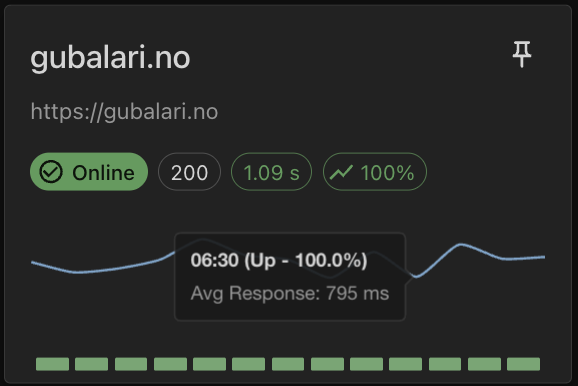
\includegraphics[width=1\linewidth]{figures/final_application/tooltip_responsetime_chart_card.png}
    \caption{Updated Website Card}
    \label{fig:updated_web_card}
\end{figure}

\paragraph{Back Button}
The need for an explicit return path from the subpages, such as Website Details, to the dashboard was identified in user test 2. Addressing the lack of intuitivity of the system, NF.3, the final application includes a dedicated back button in the header of subpages (Figure~\ref{fig:header_websitedetails}).

\begin{figure}[H]
    \centering
    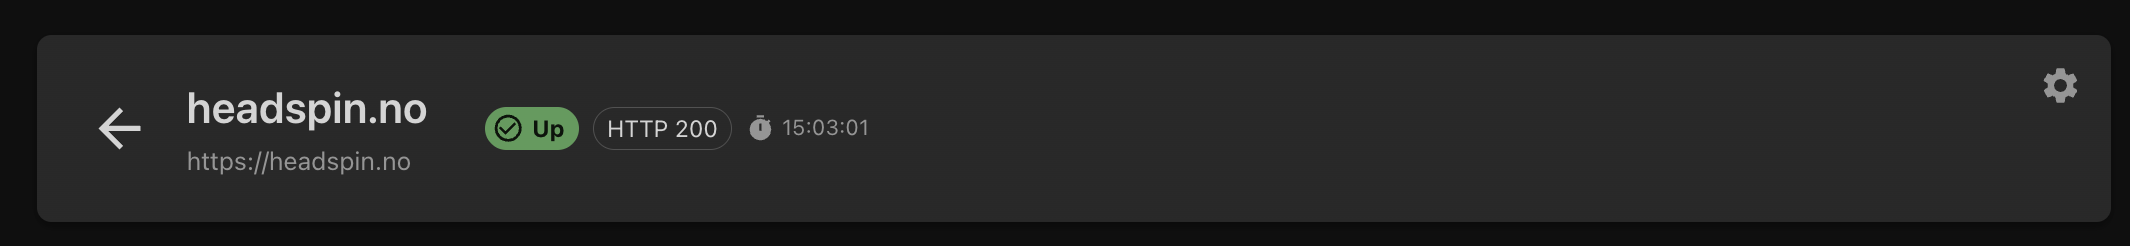
\includegraphics[width=1\linewidth]{figures/header_websiteDetails.png}
    \caption{Website Details Header with back-button, status indicators, and cogwheel for settings}
    \label{fig:header_websitedetails}
\end{figure}

Further addressing the intuitiveness of the dashboard, a designated "Add Website" card was introduced in the final delivery. This addition centralized the process of adding new websites, ensuring that critical functionality was accessible from multiple points in the interface. The implementation of this feature can be seen in Figure~\ref{fig:addwebsitecard}.

\begin{figure}[H]
    \centering
    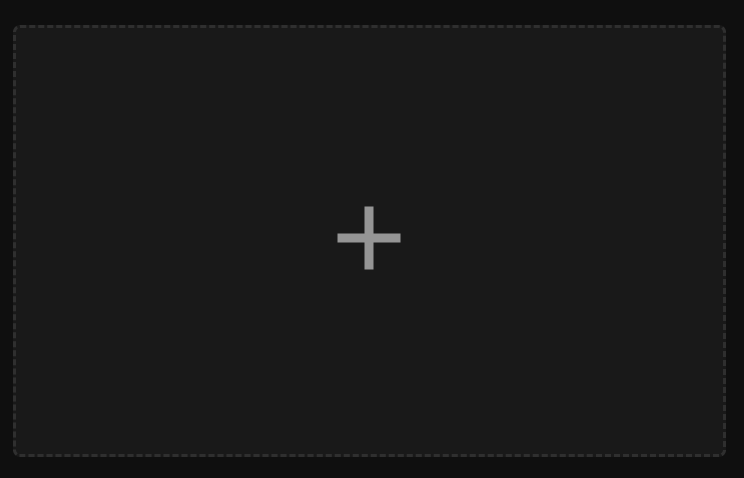
\includegraphics[width=0.5\linewidth]{figures/addwebsitecard.png}
    \caption{Add Website Card}
    \label{fig:addwebsitecard}
\end{figure}

\paragraph{New Status Banner}
P1 noted that the status banner introduced in the MVP took up to much vertical space. While providing important information, it limited how many website cards that could be displayed. In response to this,  strenghtening the fulfilment of requirement NF.3 of making website status eay to interpret at a glance, the status banner, TV-Mode, search bar, and filter options were consolidated into a single, compact component (Figure~\ref{fig:statusbar}). 

\begin{figure}[H]
    \centering
    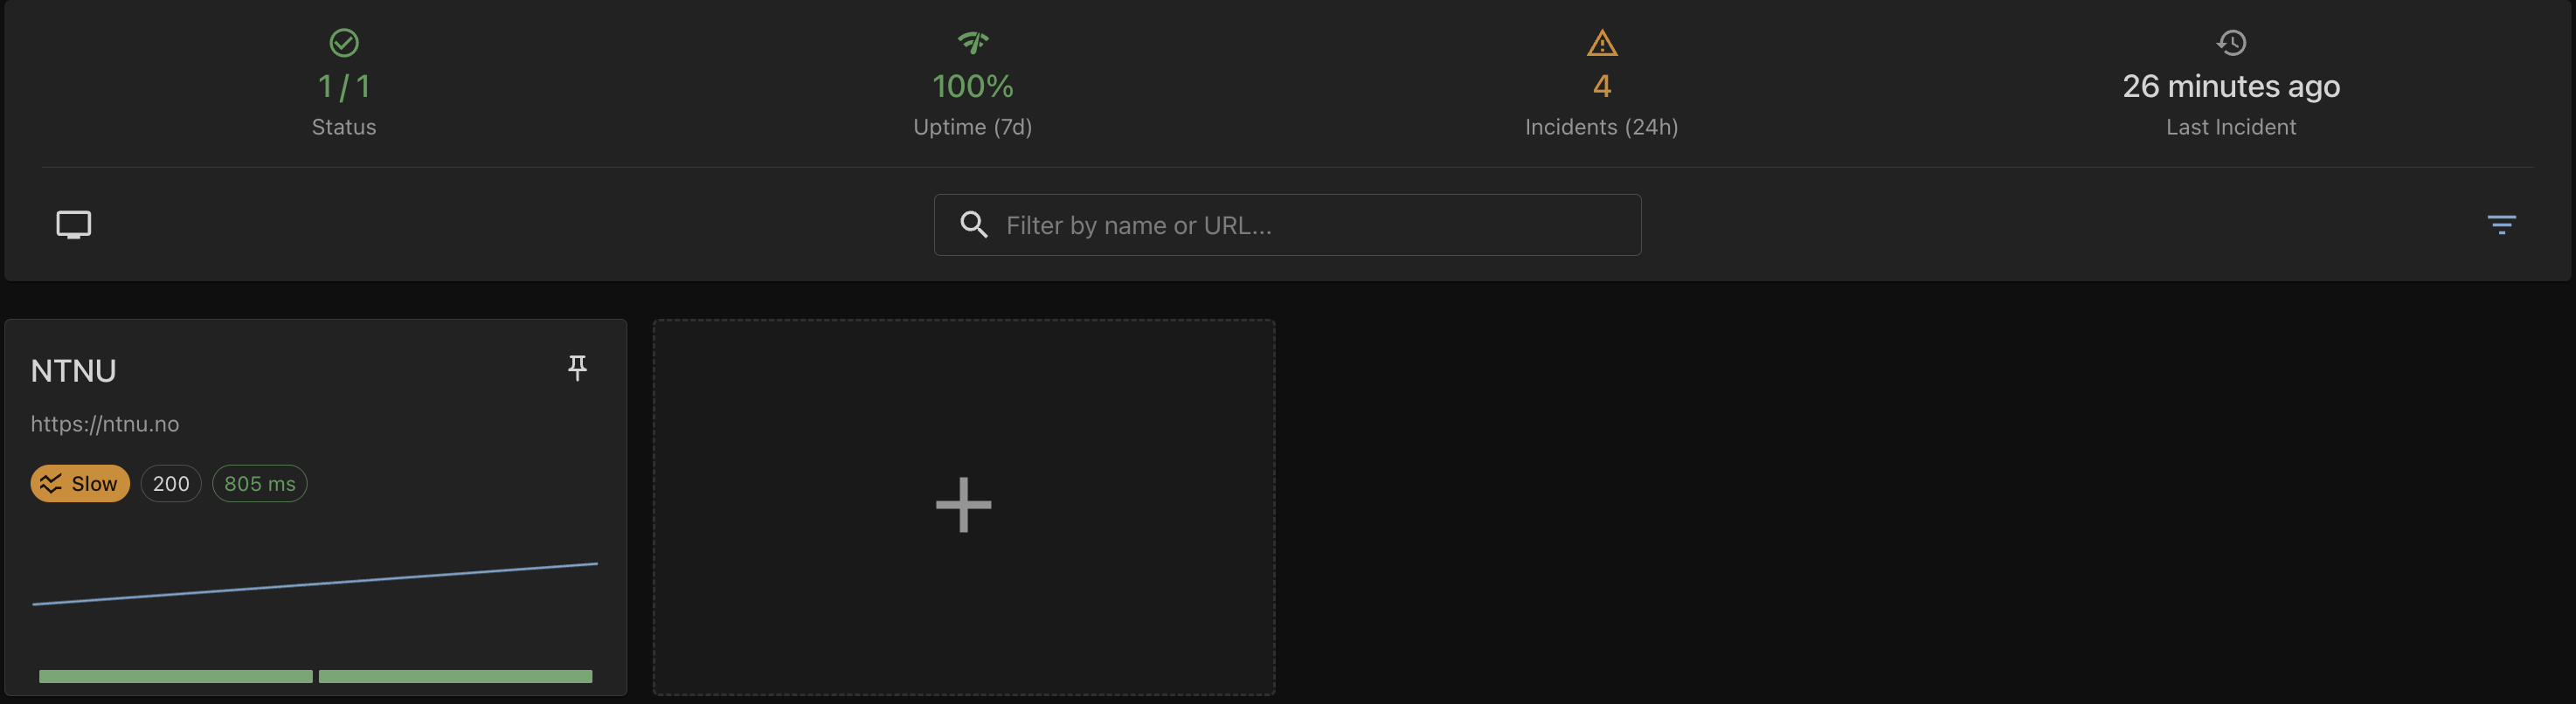
\includegraphics[width=1\linewidth]{figures/statusbar.png}
    \caption{Status Banner with TV-mode, Search bar and Filtering}
    \label{fig:statusbar}
\end{figure}


\paragraph{TV-Mode}
The feature, originally labeled “Focus-mode,” was renamed and its design was revised following feedback from user test 2. As shown in Figure~\ref{fig:tv-mode}, TV-mode activates a fullscreen display which hides both the navbar and filter bar, thereby prioritizing the display of status cards. The icon and tooltip for TV-mode were redesigned after user test 2.



\begin{figure}[H]
    \centering
    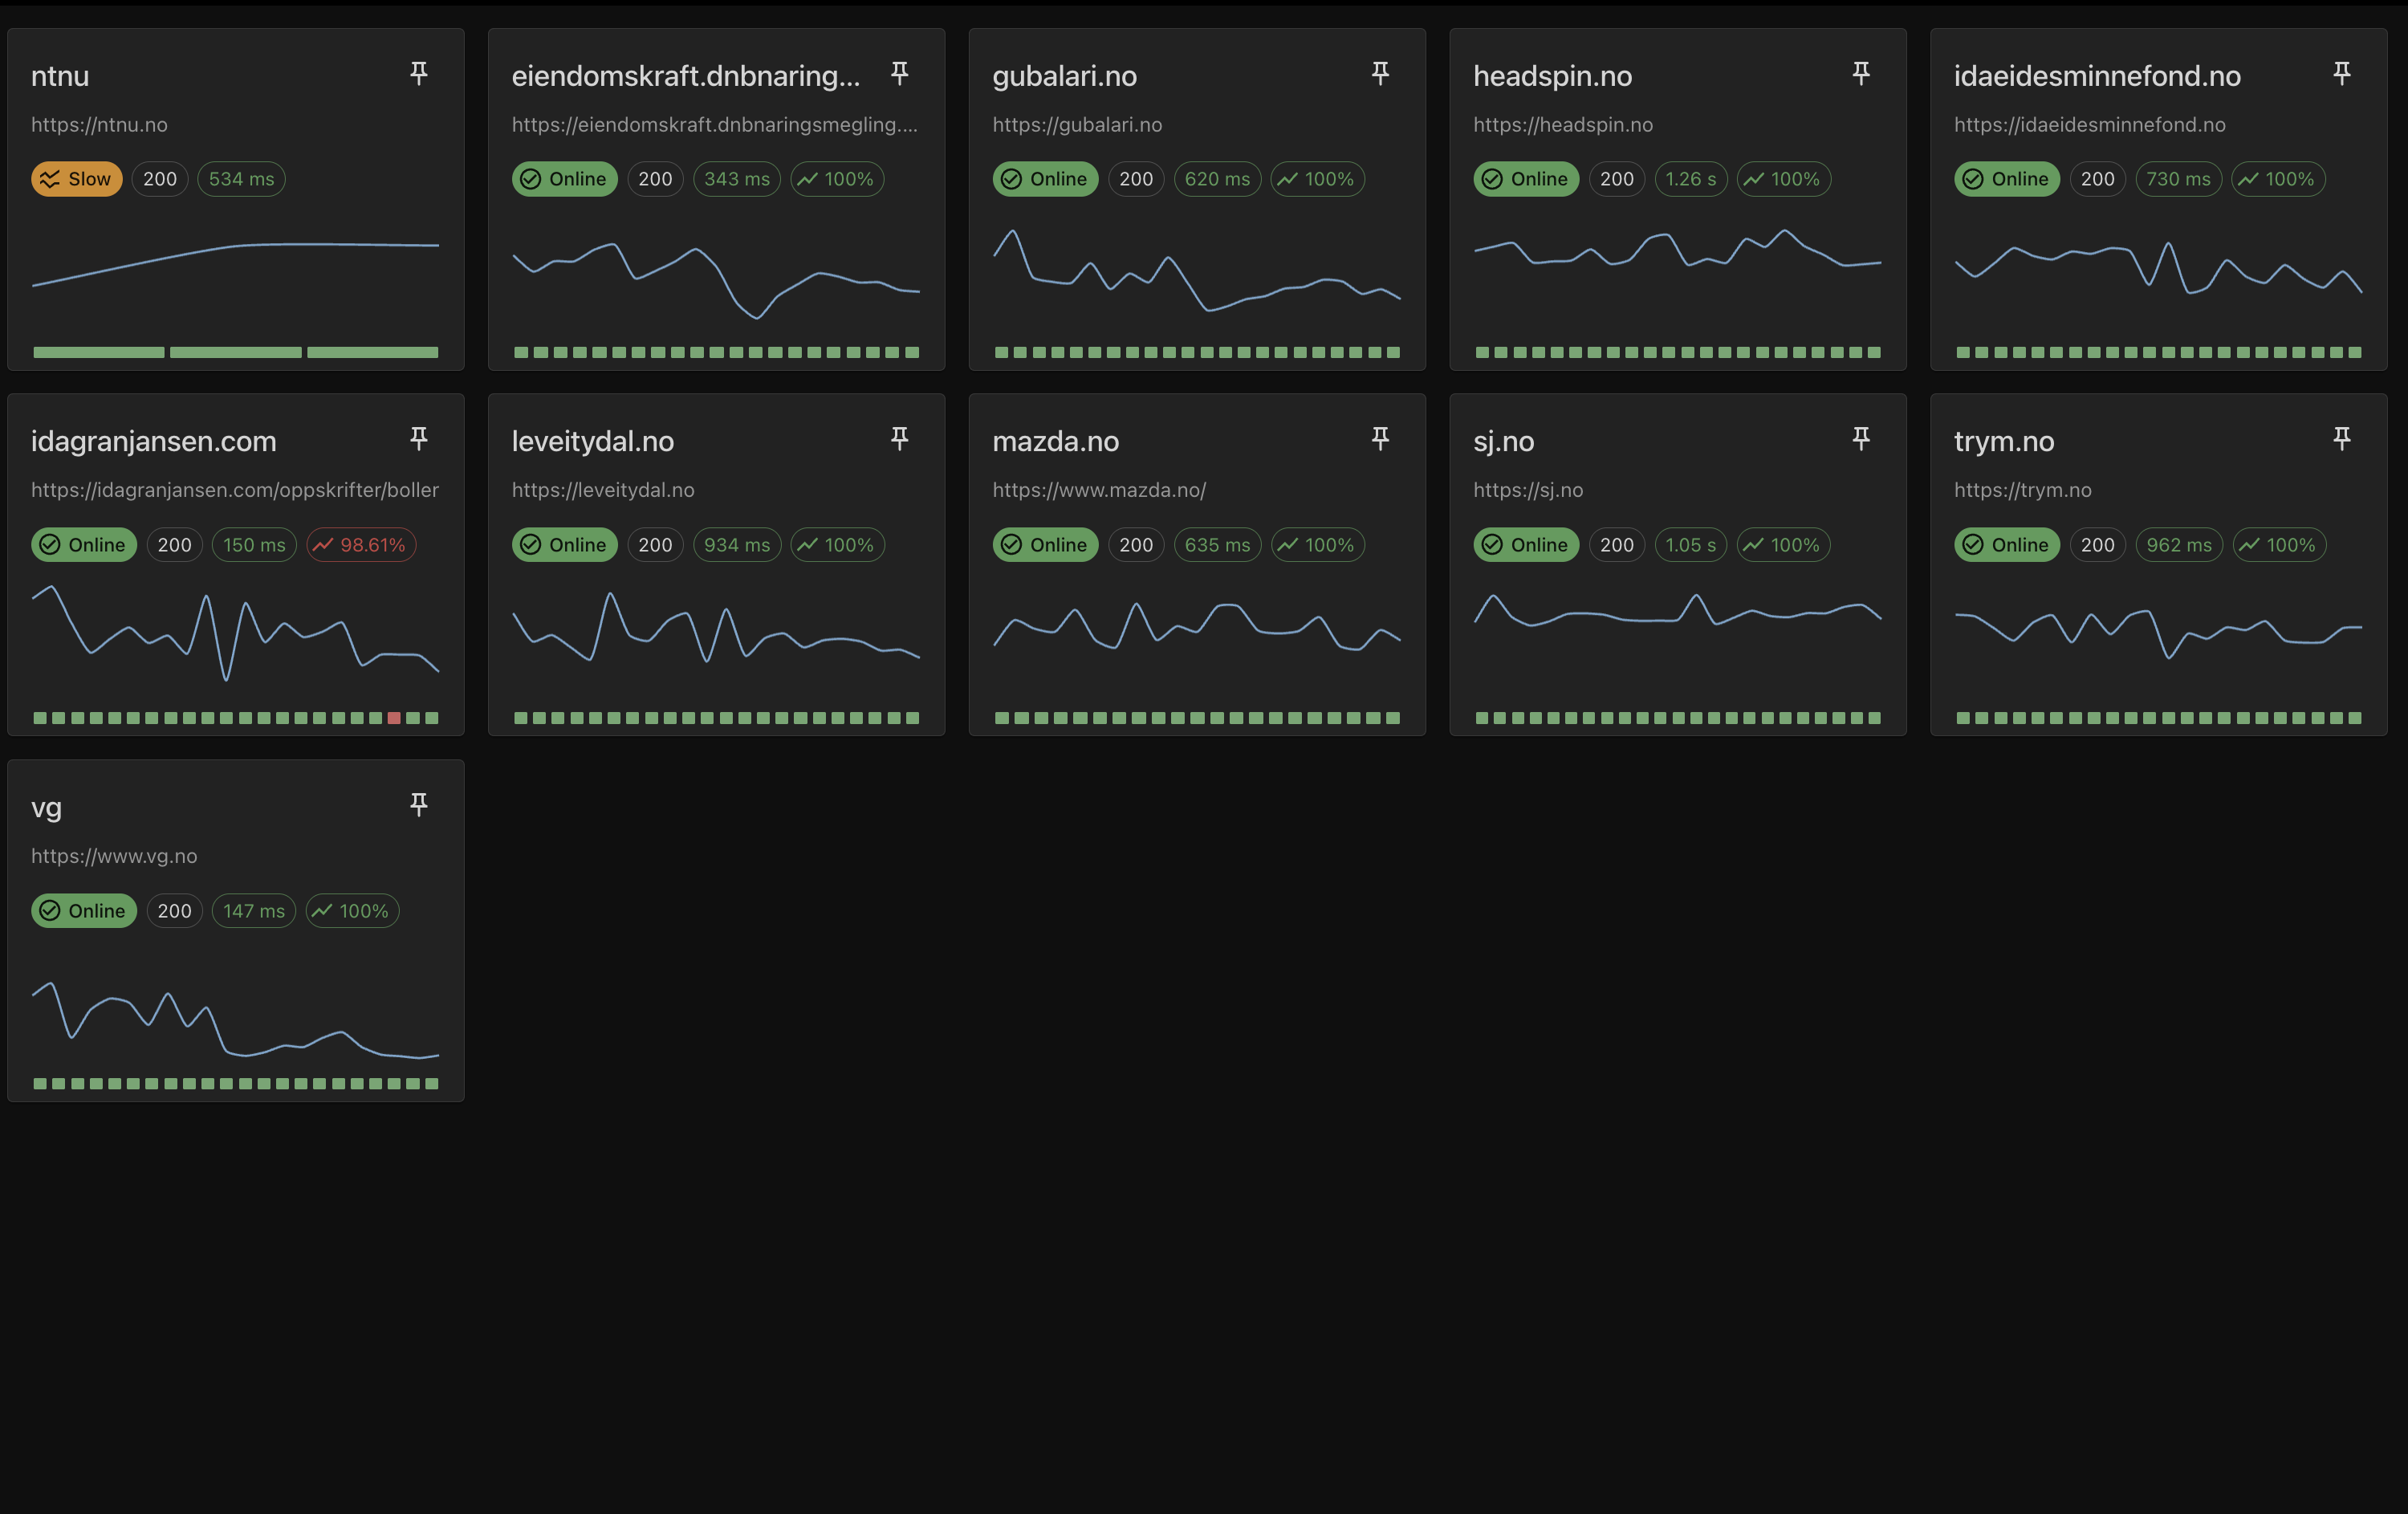
\includegraphics[width=0.75\linewidth]{figures/tv-mode.png}
    \caption{TV-Mode}
    \label{fig:tv-mode}
\end{figure}



%Gammel del


%Final product status skal inneholde en oppsumering av hvordan dashboard designet endte opp, med figure som viser produktet, før man så viser sitemap
% ting som ikke har blitt visit frem:
%overall dashboard
%



\subsubsection{Final Product Status}
After implementing the changes based on feedback and refining for requirements, the application is now in its final stage. In this section we will introduce the final version in its totality, ranging from final design and how the system works and performs.


\paragraph{Dashboard Page Design}
The main dashboard (Figure~\ref{fig:main_dashboard}) was designed applying Few’s simplicity principle and Nielsen’s aesthetic and minimalist heuristic. Information presentation includes dynamic component ordering based on website status, iconography, and colour-based status indicators. Gestalt principles, including proximity, enclosure, and similarity, were applied to the layout of elements (as shown in Figure~\ref{fig:main_dashboard}), with the intention of improving visual organization and structure.

\begin{figure}[H]
    \centering
    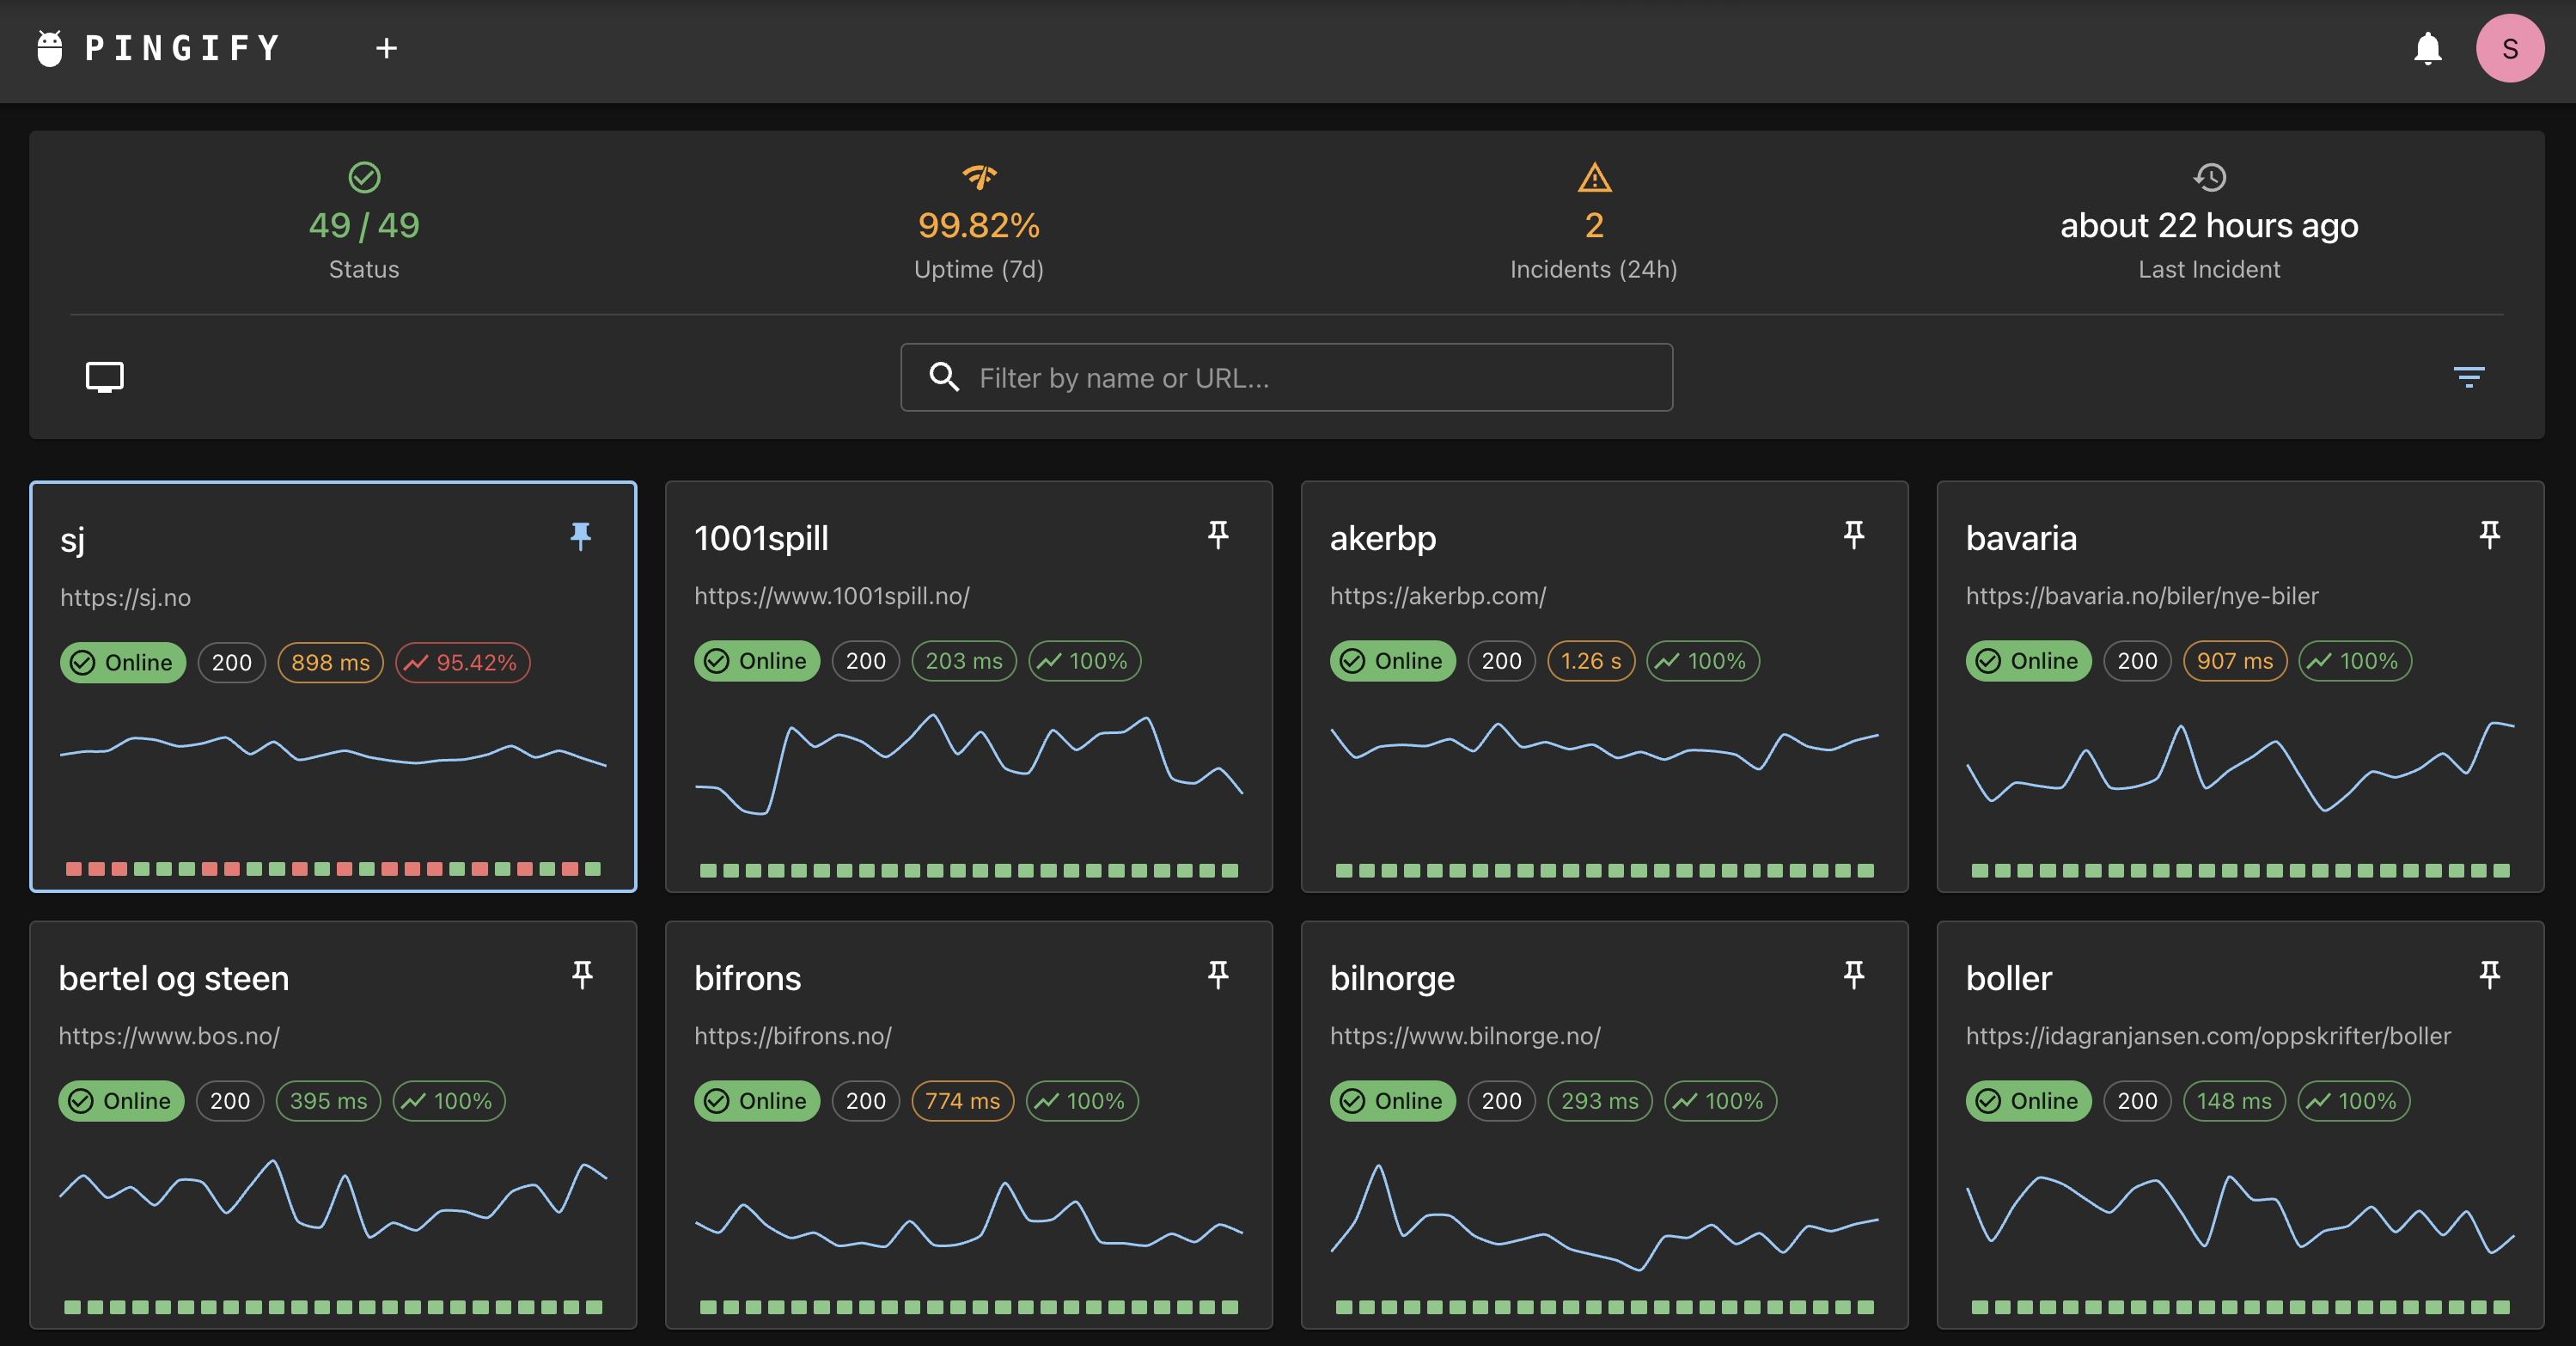
\includegraphics[width=1\linewidth]{figures/main_dashboard.png}
    \caption{Main Dashboard with Pinned Website}
    \label{fig:main_dashboard}
\end{figure}


\paragraph{System Architecture and Implementation Components}

This section presents key components of the application’s architecture that were central to its development. These include the final sitemap, database schema, system monitoring logic, and selected diagrams used to document interactions. Together, they show how the technical foundation of the system was structured and how the implementation evolved over time.

The sitemap in Figure~\ref{fig:sitemap_final} shows the structure of the application, including the different pages and how they are connected. It reflects the final design of the system after multiple iterations and testing cycles, and illustrates how users navigate between main areas such as the dashboard, website details, and the incident list.

\begin{figure}[H]
\centering
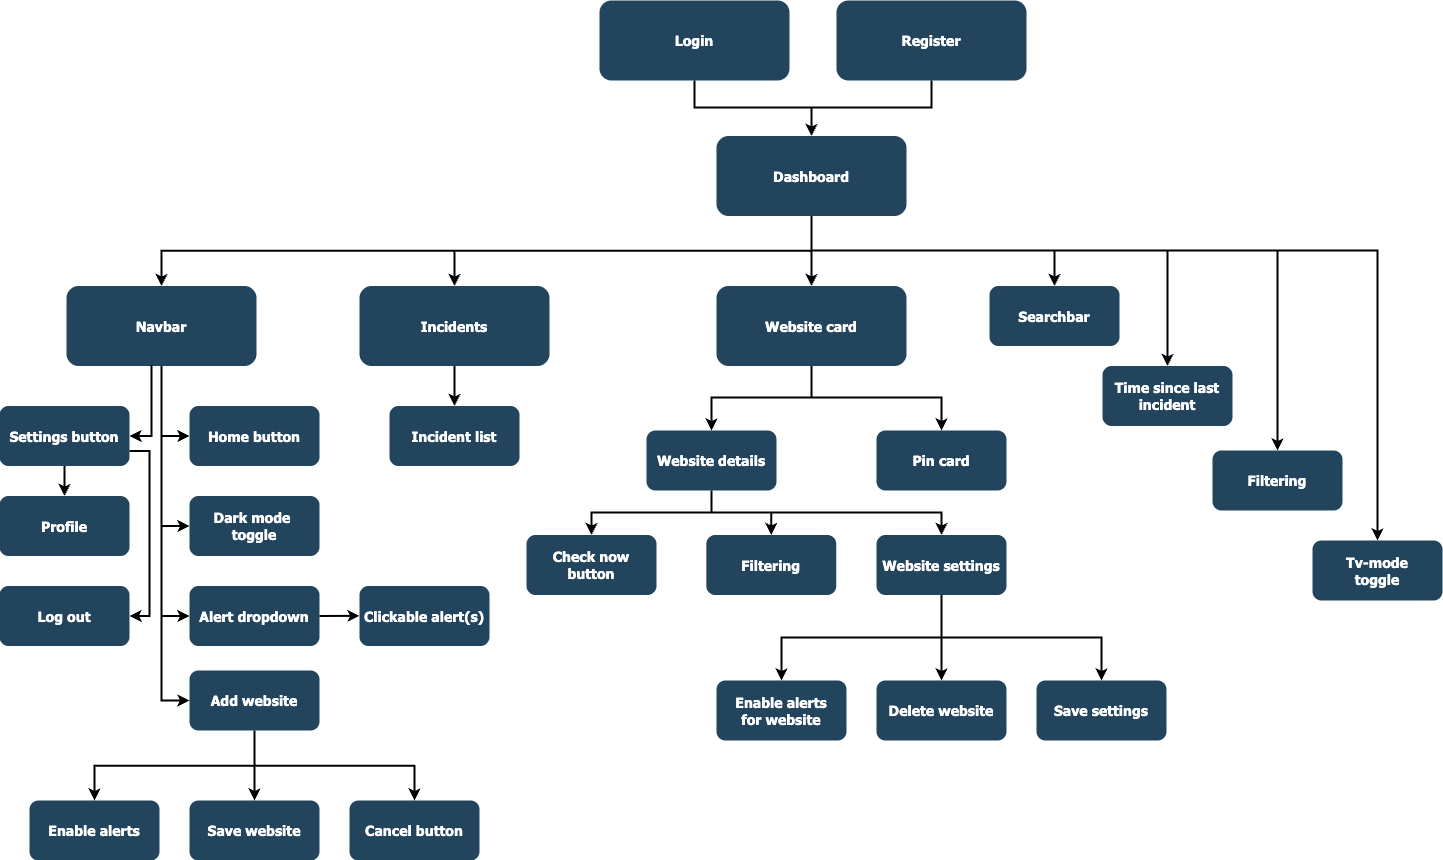
\includegraphics[width=\textwidth]{figures/diagrams/sitemap-final.png}
\caption{Final sitemap of the application structure and page relationships}
\label{fig:sitemap_final}
\end{figure}

\paragraph{Database Schema and Entity Design}

The backend of the application is built on a MySQL database. The database schema, shown in Figure~\ref{fig:er_schema_results}, was updated throughout development as new features were added. One of the key changes was the introduction of a separate table for tracking incidents, which replaced an earlier design where incidents were tied directly to alerts. This made it possible to track ongoing issues more accurately, even when alerts were dismissed.

The schema includes other important tables such as:
\begin{itemize}
    \item \texttt{User}: storing account information,
    \item \texttt{Website}: containing monitored site data,
    \item \texttt{MonitoringResult}: holding check results like response time,
    \item \texttt{Website\_Users}: connecting users with the websites they monitor, and allowing settings like custom intervals and alert preferences.
\end{itemize}

\begin{figure}[H]
\centering
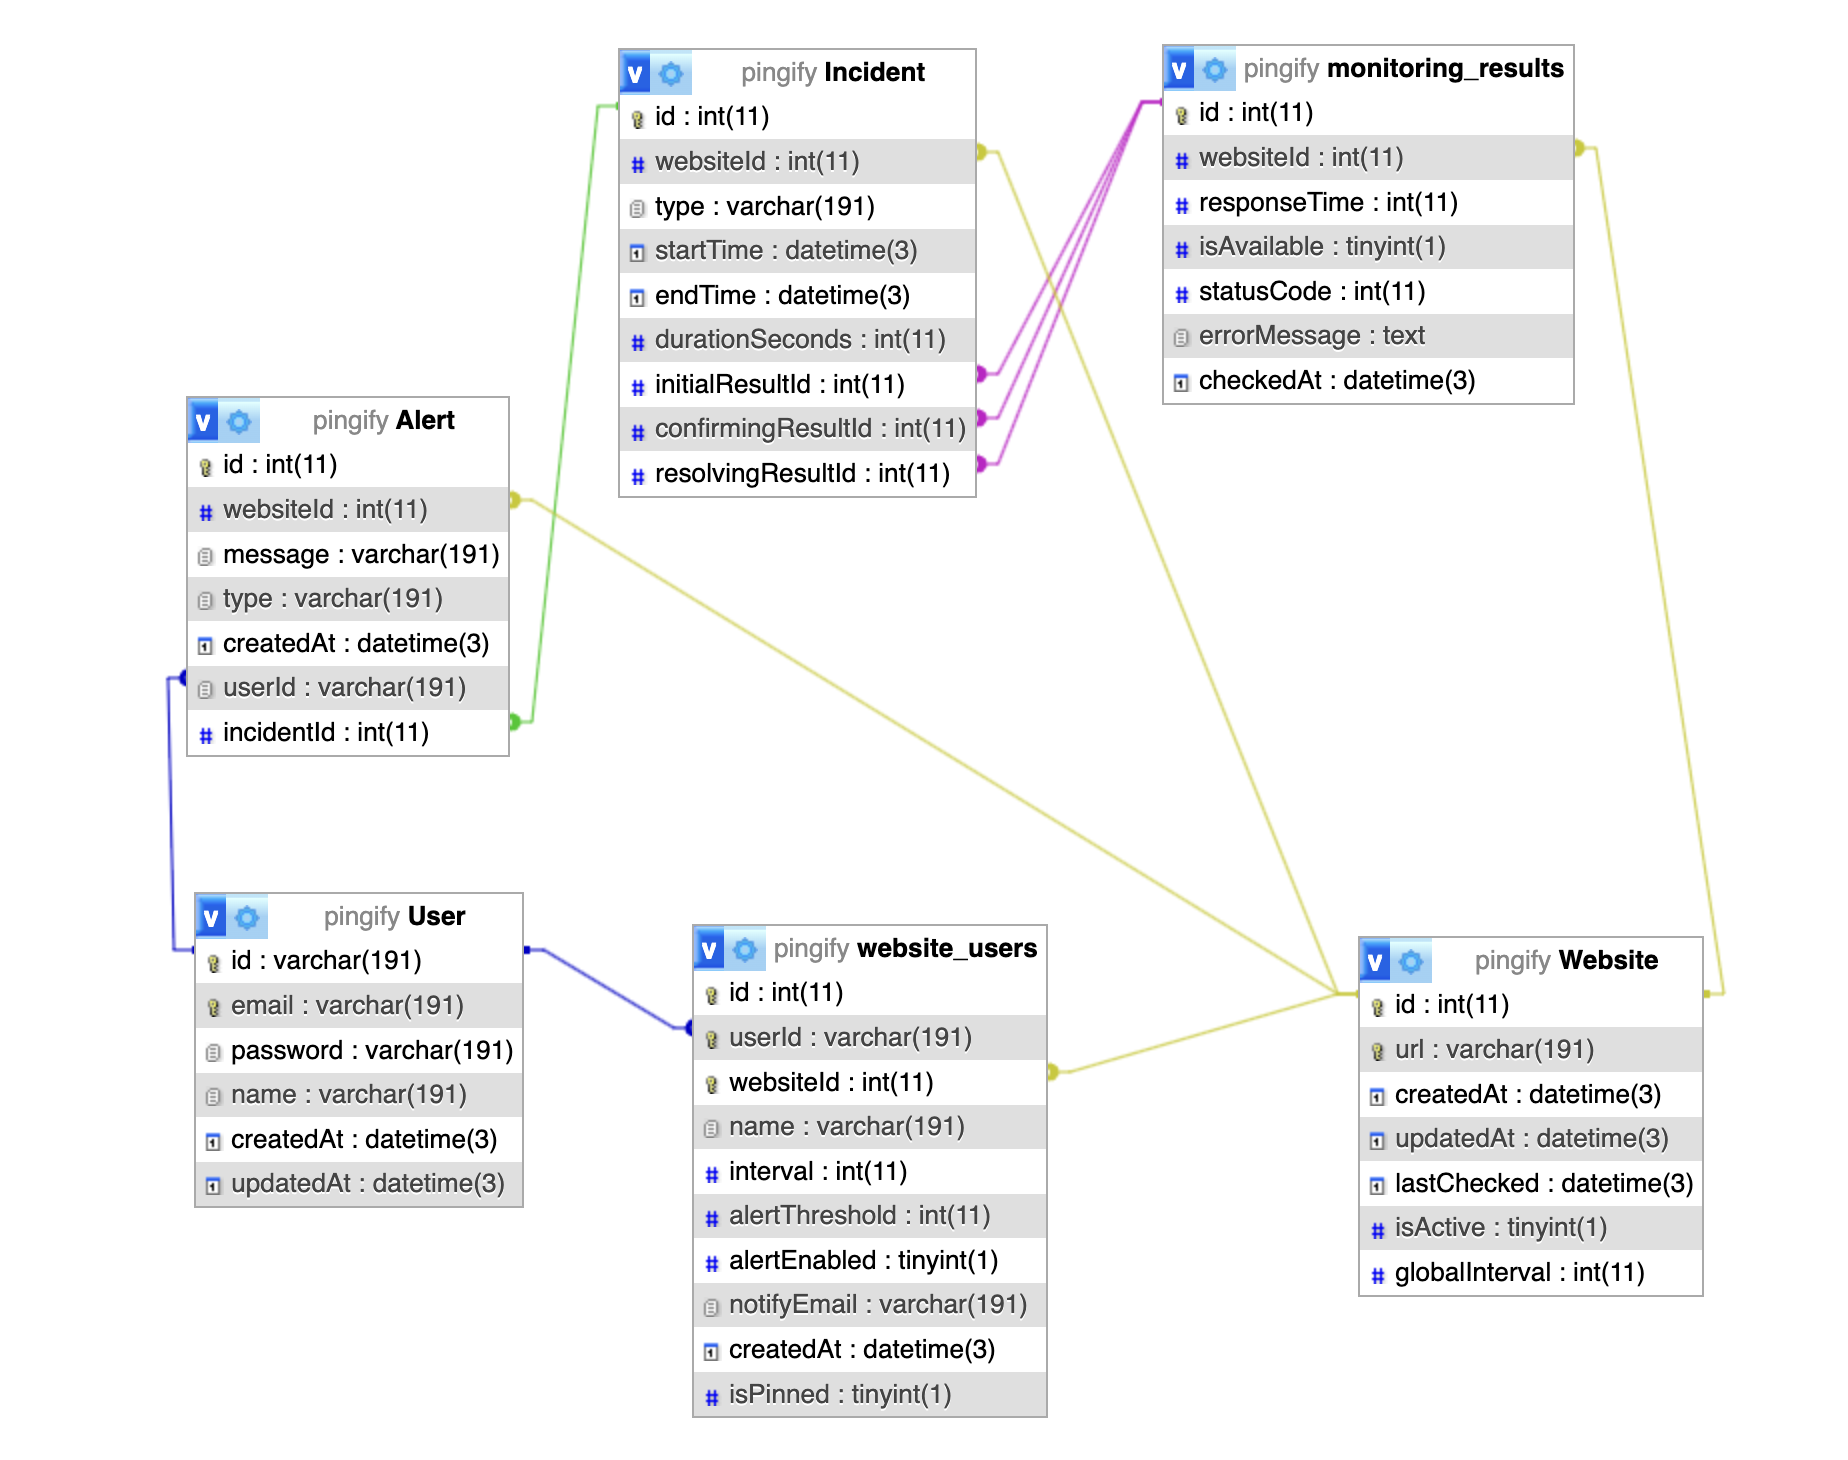
\includegraphics[width=0.85\linewidth]{figures/diagrams/mysql_scheme.png}
\caption{Final MySQL schema of the application, updated after user test 2 to include persistent incident tracking}
\label{fig:er_schema_results}
\end{figure}

\paragraph{Frontend--Backend Interaction Flow}

Figure~\ref{fig:sequence_website_details} shows how the system responds when a user clicks on a website card in the dashboard. This action sends a request through the frontend to the backend, which then fetches the relevant data from the database. The data is returned to the frontend and displayed on the Website Details page. Although this diagram was created after the implementation, it represents one of the most frequently used flows in the system.

\begin{figure}[H]
\centering
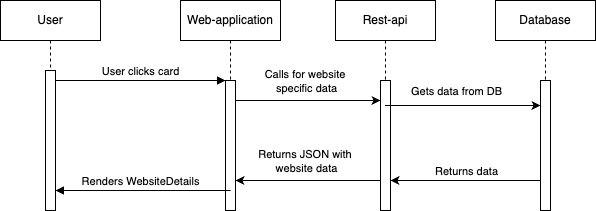
\includegraphics[width=0.9\linewidth]{figures/diagrams/Sequence_diagram.jpg}
\caption{Sequence diagram showing data flow when a user opens the Website Details page}
\label{fig:sequence_website_details}
\end{figure}

\paragraph{Monitoring Logic and Scheduling}

Monitoring the status of websites is one of the core functions of the application. This was implemented using two main tools:
\begin{itemize}
    \item \texttt{Axios}, which sends HTTP requests to the websites,
    \item \texttt{Cron}, which schedules when these requests are made.
\end{itemize}

Each monitored website is checked at regular intervals, either based on a global setting or on custom settings defined by the user. The check records whether the website is reachable, how long it takes to respond, and what status code it returns. These results are saved in the database and used to display up-to-date information in the dashboard.

To avoid performance issues when monitoring many websites at once, the system checks websites in small groups, known as batches. Each batch is processed in parallel, with a limited number of websites checked at the same time. This method prevents the system from sending too many requests at once and keeps it stable under load. The batch monitoring process is illustrated in Figure~\ref{fig:batch_monitoring_diagram}.

\begin{figure}[H]
    \centering
    \scalebox{0.7}{
    \begin{tikzpicture}[node distance=1.2cm and 2.2cm, every node/.style={align=center}]
        % Nodes
        \node (start) [draw, rectangle, rounded corners] {Cron scheduler\\triggers monitoring};
        \node (fetch) [draw, rectangle, below of=start] {Fetch active websites\\from database};
        \node (filter) [draw, rectangle, below of=fetch] {Filter websites\\due for checking};
        
        \node (batch1) [draw, rectangle, below left=2.2cm and 4.5cm of filter] {Batch 1:\\Site A, Site B};
        \node (batch2) [draw, rectangle, below of=filter, yshift=-2.8cm] {Batch 2:\\Site C, Site D};
        \node (batch3) [draw, rectangle, below right=2.2cm and 4.5cm of filter] {Batch 3:\\Site E, Site F};

        \node (db1) [draw, rectangle, below of=batch1, yshift=-0.3cm] {Results saved\\to database};
        \node (db2) [draw, rectangle, below of=batch2, yshift=-0.3cm] {Results saved\\to database};
        \node (db3) [draw, rectangle, below of=batch3, yshift=-0.3cm] {Results saved\\to database};

        \node (done) [draw, rectangle, below of=filter, yshift=-8.8cm] {All due websites\\checked};

        % Arrows
        \draw[->] (start) -- (fetch);
        \draw[->] (fetch) -- (filter);
        \draw[->] (filter) -- (batch1);
        \draw[->] (filter) -- (batch2);
        \draw[->] (filter) -- (batch3);
        \draw[->] (batch1) -- (db1);
        \draw[->] (batch2) -- (db2);
        \draw[->] (batch3) -- (db3);
        \draw[->] (db1) -- (done);
        \draw[->] (db2) -- (done);
        \draw[->] (db3) -- (done);
    \end{tikzpicture}}
    \caption{Batch-based monitoring process using scheduled tasks and grouped website checks}
    \label{fig:batch_monitoring_diagram}
\end{figure}






\subsection{Quantitative Usability Evaluation (SUS Scores)}
\label{subsec:quant_sus}
After user test 2, all three participants completed the \acrshort{sus} form immediately after finishing their tasks, and before any debriefing took place. Their individual scores are shown in Table~\ref{tab:sus-scores}.

The following table shows the score of each participant scored according to the calculation guide from 

\begin{table}[H]
\centering
\begin{tabular}{@{}lccccccccccc@{}}
\toprule
\textbf{Participant} & \textbf{1} & \textbf{2} & \textbf{3} & \textbf{4} & \textbf{5} & \textbf{6} & \textbf{7} & \textbf{8} & \textbf{9} & \textbf{10} & \textbf{SUS} \\
\midrule
User 1 & 4 & 2 & 4 & 1 & 4 & 2 & 4 & 2 & 4 & 2 & 77.5 \\
User 2 & 4 & 2 & 4 & 2 & 4 & 1 & 5 & 1 & 4 & 1 & 85.0 \\
User 3 & 5 & 1 & 5 & 1 & 4 & 2 & 5 & 2 & 5 & 1 & 92.5 \\
\midrule
\textbf{Mean} &  &  &  &  &  &  &  &  &  &  & \textbf{85.0} \\
\bottomrule
\end{tabular}
\caption{Individual \acrshort{sus} item ratings and overall scores}
\label{tab:sus-scores}
\end{table}


The resulting mean \acrshort{sus} score of \textbf{85.0} places the MVP of the dashboard well above the standard industry benchmark of 68, which is commonly interpreted as the threshold for acceptable usability \autocite{MeasuringSUS2011}. According to SUS benchmark data~\autocite{Bangor2009}, a score of 85 falls into the 95–97\textsuperscript{th} percentile, corresponding to a “B” grade and indicating excellent usability. This score was recorded after iterative design changes described in Section~\ref{sec:rq1}.

\begin{figure}[H]
    \centering
    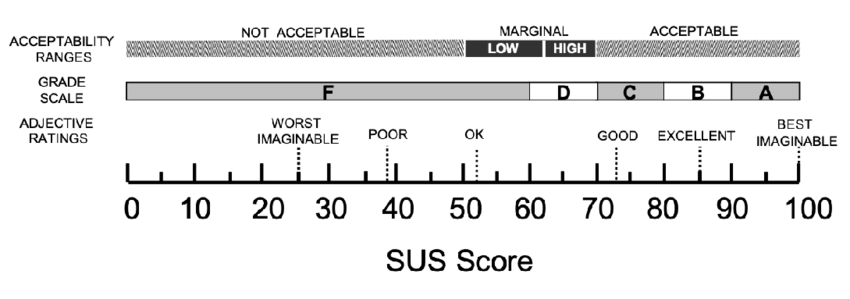
\includegraphics[width=0.8\textwidth]{figures/Grade-rankings-of-SUS-scores-from-An-Empirical-Evaluation-of-the-System-Usability.png}
    \caption{SUS Grade Rankings (adapted from \cite{Bangor2009})}
    \label{fig:sus_scores}
\end{figure}



\subsection{Universal Design}
\label{sec:universal_design}

Non functional requirement NF.5, adhering to universal design principles, was deemed low priority in this project, as the application mainly functions as an internal tool for Headspin. However, some features were implemented to support universal design, with the aim of improving accessibility and usability across a broad range of users and devices. These features contribute to the partial fulfilment of requirement NF3 (\autoref{tab:stakeholder_nonfunc_res}), which states that the interface must be user friendly and intuitive. 

\begin{itemize}
    \item \textbf{Colourblind mode}: An optional colour-blind mode was added to improve visual accessibility. This mode adjusts the default colour scheme to enhance contrast and distinguishability for users with colour vision deficiencies. Examples of the modified interface are included in Appendix~\ref{app:colourblind_mode}.

    \item \textbf{Keyboard accessibility}: The dashboard supports navigation and interaction using only the keyboard. All form elements, buttons, and navigation components are operable using standard keys such as \texttt{Tab}, \texttt{Enter}, and \texttt{Escape}. Focus indicators and consistent tab order were maintained using accessible UI components.

    \item \textbf{Responsive design}: The layout and components of the dashboard are designed to adapt to various screen sizes and resolutions, including mobile phones, tablets, and widescreen monitors. Content remains readable and interactive across breakpoints, supporting use on different devices without requiring interface adjustments.
\end{itemize}

Some accessibility aspects, such as full screen reader support and contrast testing for all visual states, were outside the project scope and are candidates for future work.



\subsection{Requirement Fulfilment Overview}
\label{subsec:req_final}

To assess whether the system met its intended functional and quality goals, this section reviews the extent to which the defined requirements were fulfilled. A total of eighteen requirements—twelve functional (F) and six non-functional (NF)—were tracked from the initial brief to the final release (see \autoref{app:req_from_brief}–\autoref{app:req_mvp_user_test}).

To support clarity and post-project analysis, the requirements are grouped below into (i) those fully implemented in the delivered system and (ii) those partially fulfilled or deferred for future work.

\begin{table}[H]
\centering
\begin{tabular}{|l|p{0.60\linewidth}|c|}
\hline
\textbf{Req.\ ID} & \textbf{Requirement (functional \& non-functional)} & \textbf{Priority}\\ \hline
F.1  & User can add, edit and delete monitored websites via the user interface.& High   \\ \hline
F.2  & User can set custom check intervals per website.& High   \\ \hline
F.3  & Display status, response time, and uptime history for each website on its dashboard card.& High   \\ \hline
F.5& Trigger alerts and notifications via e-mail or sms& Medium \\ \hline
F.6& Implement user authentication with personalised dashboards.& Medium \\ \hline

F.7  & Add functionality for filtering and sorting of website cards.& Medium \\ \hline
F.8  & Implement per-website overivew of historical data& High   \\ \hline
F.9  & Let users pin websites to the top of the dashboard.& Medium \\ \hline
F.10 & User-configurable alert thresholds for performance.                      & Medium \\ \hline
F.11 & Incident tracking system with incident list.                             & Medium \\ \hline
F.12 & Users can click on incident on graph to jump to related check.& Medium \\ \hline 
 F.13& Sparkline with status indication below response time chart on cards.&Medium \\\hline \hline
NF.1 & Monitoring of 50+ sites without noticeable delay.                        & High   \\ \hline
NF.2 & Real-time status updates with clear visual change indicators.            & High   \\ \hline
NF.6 & Card colours revised to reduce visual overload while preserving clarity. & High   \\ \hline
NF.6 & Dashboard data refreshes in near real-time.               & High   \\ \hline
\end{tabular}
\caption{Requirements fully implemented in the final system}
\label{tab:req_complete}
\end{table}

\begin{table}[H]
\centering
\begin{tabular}{|l|p{0.55\linewidth}|c|c|}
\hline
\textbf{Req.\ ID} & \textbf{Requirement} & \textbf{Priority} & \textbf{Status}\\ \hline
F.4  & Verify end-to-end page integrity beyond HTTP 200. & High & Unmet \\ \hline 
F.14 & Incident list and last incident buttons visible on status banner.& Low&Unmet\\ \hline 
F.15 & Title and legend on card chart& low&Unmet\\\hline\hline \hline
NF.3 & Interface universally user-friendly and fully responsive. & High & Partial \\ \hline
NF.4 & Maintainable, fully documented code base. & Medium & Partial \\ \hline
\end{tabular}
\caption{Requirements partially implemented or deferred}
\label{tab:req_incomplete}
\end{table}

\paragraph{Coverage}
\begin{itemize}
    \item \textbf{Fully implemented:} 16 of 21 requirements ($\approx$76\%)—including 12 functional and 4 non-functional.
    \item \textbf{Partially implemented or unmet:} 5 of 21 requirements ($\approx$24\%)—deferred or incomplete.
\end{itemize}

\paragraph{Notes on partially implemented or unmet items}
\begin{itemize}
    \item \textbf{F\,4 — Page integrity checks:} Not implemented. Verifying end-to-end content beyond HTTP~200 was deprioritised due to technical complexity.
    \item \textbf{F\,14 — Incident header actions:} The incident list and shortcut buttons intended for the status banner remain unimplemented.
    \item \textbf{F\,15 — Graph titles and legends:} Graphs for downtime and performance lack descriptive titles and legends at project hand-off.
    \item \textbf{NF\,3 — Responsive usability:} The interface is optimised for desktop and tablet; further testing and improvements are required for mobile and assistive technologies (e.g., screen readers).
    \item \textbf{NF\,4 — Maintainability:} The system includes inline documentation and a project README; however, a full developer guide and API documentation remain incomplete.
\end{itemize}

\paragraph{Project Outcome and Iterative Impact}
The final system fulfills approximately 76\% of all defined requirements, including all core monitoring, alerting, and dashboard functionality prioritised by Headspin. Iteratively developed features—such as filtering and pinning (F7, F9), configurable alerts (F10), and the incident tracking system (F11)—demonstrate how user and stakeholder feedback directly shaped the system. Partially fulfilled or unmet requirements reflect deliberate trade-offs made to deliver a stable and usable MVP. These outstanding items now serve as a clear foundation for future development, as discussed in Chapter~\ref{ch:discussion}.



\section{Summary of Key Findings}
This chapter has presented results structured around the two main research questions.

Iterative application of design principles—particularly those by Few, Norman, and Nielsen—led to targeted interface improvements including revised colour schemes, enhanced visual hierarchy, and navigation refinements. These changes were guided by usability testing, and their impact is reflected in the recorded mean System Usability Scale (\acrshort{sus}) score of 85.0 for the MVP. This score places the dashboard within the 95th–97th percentile, indicating excellent usability (Figure~\ref{fig:sus_scores}).

The system evolved through successive rounds of feedback and requirement refinement. These iterations contributed to the introduction of key functionality such as filtering, configurable alerts, and incident tracking. The progression and final status of all tracked requirements are outlined in Tables~\ref{tab:req_evolution_table} and \ref{tab:req_fulfilment_matrix}, with 76\% fully implemented by project completion.

\section{Relation to Project Objectives}
The final system delivers core functionality for real-time website monitoring, user-specific dashboards, and automated incident tracking. It integrates visual and interaction design principles with technical features aligned to stakeholder priorities and the original problem statement.

While several advanced requirements remain partially or fully unmet, the delivered MVP forms a strong foundation for further development. The next chapter reflects on these findings, assesses their broader implications, and discusses limitations, trade-offs, and directions for future work.
